\documentclass[a4paper,14pt,twoside
%,draft
]{scrreprt}

\usepackage[parfill]{parskip}
\usepackage{graphicx}
\usepackage{fancyhdr}
\usepackage{eso-pic}
\usepackage{caption}
\usepackage{hyperref}
\usepackage{wrapfig}
\usepackage{menukeys}
\usepackage{url}

%\usepackage{showframe}

\usepackage{fontspec}
\usepackage{polyglossia}
\setmainlanguage{german}
\newcommand{\glqq}{„}
\newcommand{\grqq}{“}

\newcounter{linkcounter}
\newcommand\linklist{}
\makeatletter
\newcommand{\link}[1]{%
    \edef\tmptoken{\detokenize{#1}}%
    \@ifundefined{nopanic@link@\tmptoken}{%
        \protected@edef\@tmpkey{{\fontsize{13pt}{0}\selectfont\keys{\arabic{linkcounter}}}}%
        \expandafter\global\expandafter\edef\csname nopanic@link@\tmptoken\endcsname{\arabic{linkcounter}}%
        \expandafter\g@addto@macro\expandafter\linklist\expandafter{\@tmpkey & \url{#1}\\}%
        \stepcounter{linkcounter}%
    }{%
        \protected@edef\@tmpkey{{\fontsize{13pt}{0}\selectfont\keys{\csname nopanic@link@\tmptoken\endcsname}}}%
    }%
    \href{#1}{\@tmpkey}%
}
\makeatother

\definecolor{ifsrgreen}{rgb}{0.69, 0.88, 0.11} % 177, 225, 28
\definecolor{ifsrgray}{rgb}{0.6, 0.6, 0.6} % 153, 153, 153

\changemenucolor{gray}{bg}{named}{ifsrgreen} %background of the menukeys
\changemenucolor{gray}{br}{named}{white} %border of the menukeys
%\changemenucolor{gray}{txt}{named}{white} %text of the menukeys

\setmainfont{PT Sans}
\setkomafont{chapter}{\color{ifsrgreen}\fontspec[BoldFont={* Bold}]{Exo}\huge}
\setkomafont{chapterentry}{\normalfont\bfseries}
\setkomafont{minisec}{\color{ifsrgray}\fontspec[BoldFont={* Bold}]{Exo}\large}
\setkomafont{paragraph}{\color{ifsrgray}\fontspec[BoldFont={* Bold}]{Exo}}
\setkomafont{pagenumber}{\color{ifsrgray}\fontspec{Roboto}}

\sloppy % forces "ugly" line breaks

\pagestyle{plain}

\begin{document}

%Das Coverbild, oh gott o.O Aber es funktioniert
\newcommand\CoverPic{%
\put(0,0){%
\parbox[b][\paperheight]{\paperwidth}{%
\vfill
\centering

\includegraphics[width=\paperwidth,height=\paperheight,%
keepaspectratio]{cover/Vorne}%
\vfill
}}}
\thispagestyle{empty} %keine Seitenzahl
\AddToShipoutPicture*{\CoverPic}
\mbox{} %brauche leeren Content für ne newpage
%\newpage

% Wie erstellt man den Zeitplan?
% 1. man läd sich den HTML Code von ese.ifsr.de herunter
% 2. man fügt folgendes CSS manuell hinzu und bestaunt das Ergebnis:
%  *{font-size:0.99!important}
%	main {margin:0;padding:0;}
%	.row {margin:0;}
%	 header, footer, .sidebar, .panel, section h2, section p, #barrierfree-heading, #timetable-heading  {display:none;}
%	tr, td  {line-height: 1em;}
%	table tbody tr td div.table-spacer {height: 1rem;!important}
%	#content {padding:0;}
%
%	td.data {width: 20%; background: #FDC412}
% 3. man benutzt z.B. wkhtmltopdf um ein PDF daraus zu erstellen:
% wkhtmltopdf -s A4 --no-print-media-type --margin-left 0 --margin-right 0 --margin-bottom 0 --margin-top 0 ESE\ 2016\ _\ iFSR.html zeitplan.pdf
% 4. ????
% 5. Färdsch


\addchap[Zeitplan der ESE-Woche]{}
\thispagestyle{empty}

%\thispagestyle{empty} %keine Seitenzahl
%\AddToShipoutPicture*{\put(0,0){%
%\parbox[b][\paperheight]{\paperwidth}{%
\begin{center}
  \vspace*{-6.5em}
  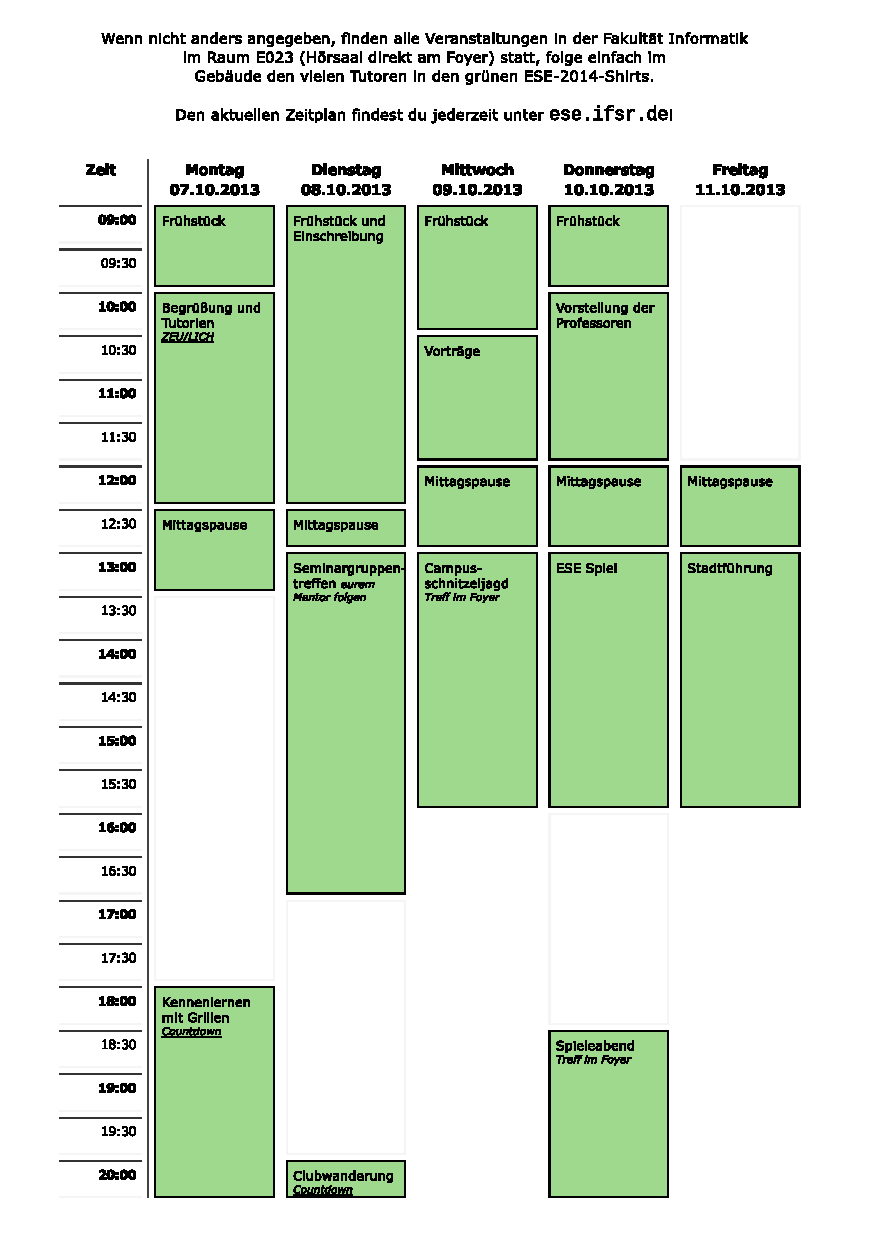
\includegraphics[height=.77\dimen108,keepaspectratio]{img/zeitplan.pdf}%
  
  \small
  \vfill
  \enlargethispage{3em}
  
  Sofern nicht anders angegeben, finden alle Veranstaltungen im Fakultätsgebäude der Informatik, dem
  \textbf{Andreas Pfitzmann Bau (APB)}, im Raum \textbf{E023} (Hörsaal direkt am Foyer) statt.
  Folge im Gebäude einfach den vielen Tutoren in den schönen, roten ESE-2018-Shirts.

  Den aktuellen Zeitplan findest du auch jederzeit unter \textbf{ese.ifsr.de} \link{https://ese.ifsr.de/}.
\end{center}

\tableofcontents
\textbf{Danke an ...}

%TODO: Tutorennamen hier einfügen
Tutor1, Tutor2, Tutor3, ...

\addchap{Vorwort}

Hallo Uniwelt!

heißt es nun für dich als frisch Immatrikulierter, Ersti, an der TU Dresden. 
Endlich kannst du nach Jahren der Knechtschaft selbst über dich und dein Leben bestimmen. 
Wie du mit dieser Freiheit und der daraus folgenden Verantwortung zurecht kommst, lernst du schnell. 
Damit dir der Übergang leichter fällt, veranstaltet dein Fachschaftsrat die Erstsemestereinführung (ESE). 
Eine Woche lang gibt es neben Spiel und Spaß sehr viel Informatives zum Studium sowie zum Unileben allgemein. 
Dieses Heft ist ein nützlicher Ratgeber und nicht vergessen: 
\textbf{NO PANIC!} (Aus historischen Gründen hier nicht das grammatikalisch korrekte \glqq don't panic\grqq. Hinweise auf diesen grammatikalischen Fauxpas werden mit Matekästenschulden geahndet.)

Du wirst auch entdecken, dass Uni mehr ist als nur studieren. 
Neben allerlei Erstsemesterparties gibt es noch mehr zu erleben. 
Gerade prägend für die Dresdner Hochschulkultur sind die 17 Studentenclubs, wie z.B. das CountDown in der Johannstadt. 
In der Neustadt laden viele Kneipen und Clubs zu langen Nächten ein. 
Einmal im Jahr entlädt sich dieses alternative Flair während der BRN (Bunte Republik Neustadt). 
Und wem das alles viel zu hektisch ist: der fläze sich gemütlich in ein Sofa vom ASCII, dem Studentencafé der Fakultät. 
Dort kann man gut bei Kaffee und Club Mate (empfehlenswert auch die lokale Kolle-Mate!) entspannen oder versuchen doch etwas für die Uni zu tun.

Engagement wird an der TU Dresden groß geschrieben. 
Es gibt viele Hochschulgruppen die um eure Mitarbeit buhlen. 
Darunter einige politische, wie auch technische, journalistische, künstlerische und und und. Mehr dazu findest du auf der Seite des StuRa.

Dieses Heft enthält übrigens auch eine Vielzahl von Links zu relevanten Unterseiten auf den Seiten des FSR, der Uni und anderen. 
Diese sind mit Zahlen wie dieser hier \link{NONE} versehen und ganz am Ende des Heftes gelistet. Ebenfalls kannst du auch direkt unter \url{ese.ifsr.de/link/XX} auf die verlinkte Seite weitergeleitet werden.
%TODO: Das sollte dann natürlich auch klappen ;)
% Link 0 bitte auf ein Nick Cage Gif weiterleiten!

\textbf{Zu guter Letzt: Wir (deine ESE-Tutoren) wünschen dir viel Erfolg und auch ordentlich Spaß beim Studium!}

\begin{figure}
\centering 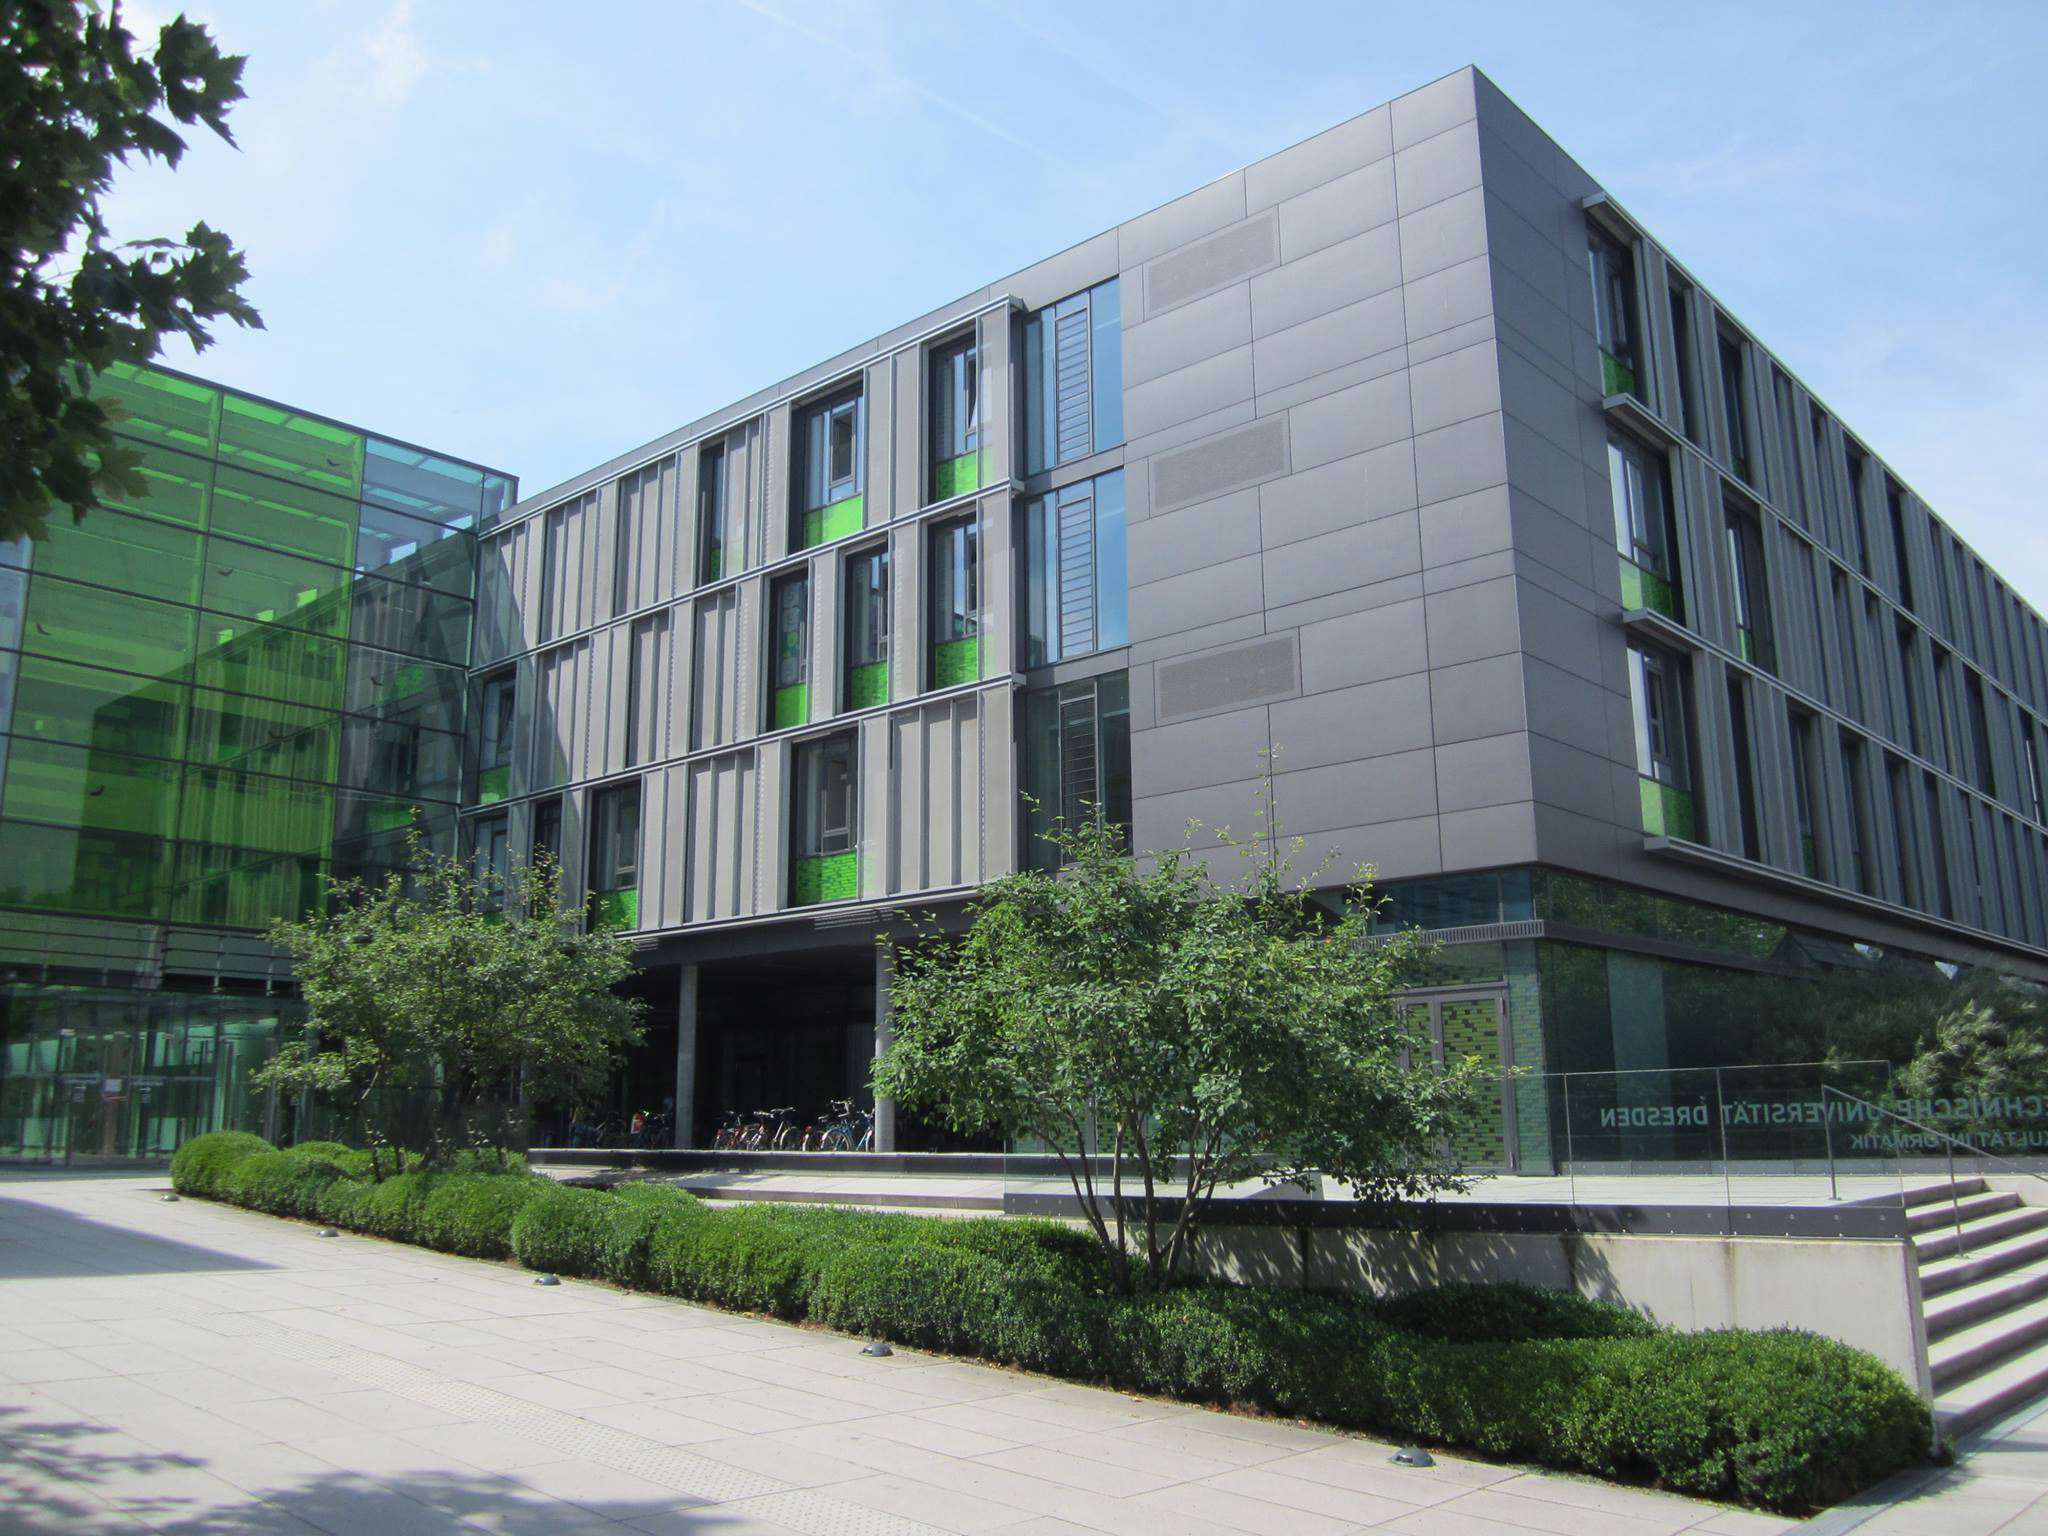
\includegraphics[width=\linewidth]{img/fakultaet.jpg}
\caption*{{\small Andreas-Pfitzmann-Bau (Fakultät Informatik) - Foto: Philipp Heisig}}
\end{figure}
%Bildlink: http://commons.wikimedia.org/wiki/File:TU-Dresden-Informatik.jpg

\thispagestyle{empty}
\AddToShipoutPicture*{\put(0,0){%
\parbox[b][\paperheight]{\paperwidth}{%
\vfill
\centering
\refstepcounter{dummy}
\label{we_want_you}
\includegraphics[width=\dimen107,height=\dimen108,keepaspectratio]{img/we_want_you.jpg}%
\vfill
}}}
\
\pagebreak

\addchap{Grußwort}

\begin{wrapfigure}{l}{0.31\textwidth}
  \vspace{-12pt}
  \begin{centering}
    
\includegraphics[width=0.3\textwidth]{img/uweassmann.png}
  \end{centering}
  \vspace{-15pt}
\end{wrapfigure}

{\fontsize{9.5pt}{11}\selectfont

Liebe Studierende,

herzlichen Glückwunsch zum Beginn eines der spannendsten Studien, die es gibt, an einer der attraktivsten Informatikfakultäten Deutschlands und Europas! Als Dekan ist es mir eine Freude, Sie herzlich an unserer Fakultät Informatik begrüßen zu dürfen. Mit 26 Professoren, 3 Honorarprofessoren, mehr als 300 Mitarbeitern und mehr als 1600 Studenten gehört die Fakultät zu den größten Informatikfakultäten Deutschlands mit einem der breitesten Spektren an Studieninhalten. Um unser modernes Gebäude werden wir von vielen anderen Fakultäten beneidet, auch wenn es manchmal mit einem Augenzwinkern als "Grünes Gewölbe" bezeichnet wird. Ich kann Ihnen aus eigener Erfahrung versichern: man gewöhnt sich an die Farbe. Das Gebäude bietet nicht nur Platz für die Mitarbeiter der Fakultät, sondern verfügt auch über einen Vorlesungssaal, diverse Seminarräume und hochwertig ausgestattete Rechner-Pools. Im Foyer liefert das Studentencafé \ascii{} den für einen Wissenschaftsbetrieb äußerst wichtigen Koffeinnachschub. Was unser Kunstwerk im Atrium bedeutet, dürfen Sie gerne raten. Hinter unserem Gebäude lädt das "Nöthnitzer Meer" zum Lernen, Chillen und Sonnen ein. Und gleich links von der Fakultät liegt unser beliebtes Sportzentrum.

Die Informatik durchdringt unsere Gesellschaft wie keine andere Wissenschaft und beschleunigt den wissenschaftlichen Fortschritt anderer Disziplinen enorm. Marc Andreesen, der Erfinder des ersten kommerziellen Web-Browsers "Netscape", prägte in 2011 den Slogan "Software is eating the world", was sagen will, dass die Digitalisierung alle Industrien und alle Lebensbereiche verändert. Software läuft nicht nur in Computern, sondern auch in Autos, Flugzeugen, Wasch- und Kaffeemaschinen. Teilweise ist der Einfluss von Software sogar so tief, dass er der Gesellschaft gar nicht mehr bewusst ist: Wer denkt heute schon darüber nach, dass sein Handy aus einem Berg voller Software besteht? Die Digitalisierung führt auch dazu, dass Firmen händeringend nach Informatikern suchen. Unsere Fakultät kann derzeit mit ihren Absolventen nicht einmal den Fachkräftebedarf der Software-Industrie im Raum Dresden decken, denn sie wächst jedes Jahr um ca. 5-7\% und benötigt dazu ca. 600 neue Informatiker. Nach dem erfolgreichen Abschluss Ihres Studiums werden Ihnen daher viele Türen offenstehen. Also zunächst einmal herzlichen Glückwunsch zu diesen guten Aussichten!

Für Sie, liebe Studentinnen und Studenten, beginnt mit dem Studium ein neuer, faszinierender Lebensabschnitt, der mehr Freiheiten bietet als die Schule vorher und das Berufsleben danach. Diese Freiheiten sollten Sie nutzen, um sich in freier Selbstbestimmung zu bilden, Ihr Studium selbst zu planen, Ihre Lerninhalte selbst zu vertiefen und sich selbst Ihre Lern-Arbeit einzuteilen. Das macht Spaß -- es bringt aber auch zwei Probleme mit sich: Erstens muss man das systematische Erarbeiten von großen Mengen an Lernstoff trainieren, und zweitens benötigt man für ein erfolgreiches Studium mehr Disziplin, als man von der Schule gewohnt ist. Also, einige Tipps: Gehen Sie bitte regelmäßig in die Vorlesungen, denn der Professor fasst dort für Sie die wichtigsten Inhalte des Fachgebiets zusammen, sodass Sie schnell Wichtiges von Unwichtigem unterscheiden können. Bereiten Sie bitte diese Kerninhalte Ihres Faches regelmäßig nach, denn dann verankern sie sich schneller in Ihrem Kopf -- nichts ist schlimmer als eine Woche Bulimie-Lernen vor der Prüfung. Schließlich: Erarbeiten Sie sich die Lösungen zu den Übungsaufgaben selbstständig, denn das selbstständige Lösen von Aufgaben führt Sie schnell zu einer höheren Stufe des Lernens und der damit verbundenen Leistungsfähigkeit (Bloomsche Lernzielhierarchie, siehe Wikipedia). Das erfolgreiche Herunterladen der Vorlesungsfolien oder des Skripts zur Vorlesung trägt nur dann zum Bestehen der Prüfung bei, wenn Sie sich auch intensiv mit den Inhalten auseinandersetzen :-) Versuchen Sie, alle Begriffe zu verstehen und zusätzlich in der Lage zu sein, sie aktiv erklären zu können. Laden Sie sich gegenseitig zum Kaffee ins \ascii{} ein und erklären Sie sich dabei, was in der letzten Vorlesung behandelt worden ist.  Das verbessert nicht nur den Studienerfolg, sondern macht auch viel mehr Spaß. (Das habe auch ich in meinem Studium so erlebt.) Und wenn Sie trotzdem im Studium auf Probleme stoßen, stehen Ihnen viele Anlaufstellen zur Verfügung: Studienberater, Mitglieder des Fachschaftsrates, Übungsgruppenleiter und selbstverständlich auch alle Professoren, die für Sie Sprechstunden anbieten, die Sie nutzen sollten, insbesondere zu einem Check vor Prüfungen.

In 2017 hat die Landesregierung die Planung des Lehmannzentrums eingeleitet, ein interdisziplinäres Zentrum für IT mit geplanten 11000 qm zusätzlicher Fläche. Es soll rechts neben dem Großrechner gebaut werden und neue "Living Labs" für die Informatik aufnehmen. Geplant sind zwei Living Labs für Immersive Visualistik, Robotic Co-Working sowie ein MakerSpace für das Internet der Dinge. Wahrscheinlich wird das Gebäude auch Platz des geplanten DLR-Softwarezentrums bieten und bereits in 2020 fertig sein. Daher sollten auch Sie in Ihrem Studium noch von den Einrichtungen des neuen Lehmannzentrums profitieren können.

Am Ende meines Grußwortes möchte ich mich ganz herzlich beim Fachschaftsrat für das große Engagement in der Fakultät und insbesondere für die Durchführung der Erstsemestereinführung bedanken. Die Fakultät lebt vom Engagement aller Mitglieder, insbesondere ihrer Studenten. Im Gegenzug bekommen Sie von uns ein vielfältiges Angebot, und das ohne Studiengebühren. Warum sollten Sie also Ihr Studium nicht als einen "ungewöhnlicherweise kostenlosen Supermarkt" betrachten, den Sie durch den "Einkaufswagen Ihres Lernens ausräumen", um später im Leben erfolgreich sein zu können? Es liegen viele spannende Themen vor uns. Gestalten Sie also mit uns die Zukunft der Informatik und mit ihr die Gesellschaft. WE WANT YOU FOR YOUR FUTURE!


\textit{Uwe Aßmann,\\
Dekan der Fakultät Informatik}

}


\addchap{Studienbetrieb}

\minisec{Die Grundbegriffe des Studiums in kurzen Worten erklärt.}

Wer \glqq frisch\grqq\ aus der Schule kommt, kennt als Lehrform vor allem den Dialog.
Üblicherweise versucht der Lehrer in der Schule, auf die Denkweise und das Arbeitstempo der Schüler einzugehen, unterhält sich mehr mit ihnen, als dass er ihnen einen Vortrag hält.
Am Ende der Stunde hat zumindest ein großer Teil der Schüler den Stoff verstanden.
An der Uni gibt es diese Lehrmethode nicht - dafür aber einige andere, an die man sich auch gewöhnen kann.
Hier wird viel Wert auf Eigenständigkeit gelegt, ein \glqq an die Hand genommen werden\grqq\ wie in der Schule, gibt es nicht mehr.
Das ist nicht die einzige Neuerung, die im Studienalltag auf dich zukommt.

\minisec{Stundenplan}

An der Uni gibt es ein so genanntes Lehrangebot, das kurz vor Beginn jedes Semesters veröffentlicht wird.
Du findest diese bereits nach Semestern sortierte Liste von Lehrveranstaltungen online auf der Seite der Fakultät \link{https://inf.tu-dresden.de/}.
Ab dem zweiten Semester besteht deine Aufgabe darin, aus dem Angebot einen Stundenplan zu basteln.
Für den Anfang bekommst du jedoch zum Eingewöhnen fertige Stundenpläne von uns, aus denen du dann einfach einen zur Einschreibung in jExam auswählen kannst.

Während Vorlesungen generell einen festen Termin haben, kannst du dich ab dem zweiten Semester flexibel in die Übungen eintragen.
Schreib dich bei jExam \link{https://jexam.inf.tu-dresden.de/} einfach für die Übungsstunden deiner Wahl ein.
Stellst du später jedoch fest, dass dein Übungsleiter die Qualitäten einer Schlaftablette aufweist oder dir die Übung zu voll ist, zögere nicht die Übung zu wechseln.


\minisec{Vorlesung}

In diesen Veranstaltungen erlebst du meistens Professoren live.
Die Zahl der Zuhörer ist in der Regel zehn Mal so groß wie die Anzahl der Schüler in einer Unterrichtsstunde. Dadurch kann natürlich nicht auf jeden Studenten eingegangen werden. Sollte dir jedoch etwas unklar sein, stelle ruhig Fragen. Oft versteht der Großteil der anderen auch nichts.
Außerdem ist es ratsam, dem Stoff stets zu folgen, da die Stoffmenge oftmals gewaltig erscheint. Sich darüber zu beschweren ist sinnlos, da der Lehrplan für die Professoren mehr oder minder vorgeschrieben ist.
Gerade deshalb hat man nur 20 Wochenstunden, da für die Nachbereitung einer Vorlesung mindestens die gleiche Zeit veranschlagt werden sollte.
Allerdings beschweren solltest du dich über schlechte Tafelbilder, undeutliche und leise Aussprache, sowie mangelnde Vorbereitung der Vorlesung. 
Professoren sind meist nicht Professoren, weil sie gute Didaktiker sind, sondern weil sie gut forschen können.
Welche Vorlesung du in welchem Semester besuchen solltest, findest du im jeweiligen Studienablaufplan deines Studiengangs (Bachelor Informatik \link{https://www.inf.tu-dresden.de/content/study/regulations/download/ba-inf/2009/study.app.2.de.pdf}, Bachelor Medieninformatik \link{https://www.inf.tu-dresden.de/content/study/regulations/download/ba-minf/2009/study.app.2.de.pdf}, Diplom Informatik \link{https://tu-dresden.de/die_tu_dresden/fakultaeten/fakultaet_informatik/studium/dateien/studien_und_pruefungsordnungen/dipl_inf_so_app1_de.pdf}) oder im Vorlesungsverzeichnis auf der Seite der Fakultät \link{https://www.inf.tu-dresden.de/index.php?node_id=2709}.


\minisec{Übungen}

Übungen werden zu fast allen Vorlesungen angeboten und dienen dazu, Aufgaben zum aktuellen Vorlesungsstoff zu bearbeiten. Klausuren orientieren sich häufig an den Übungsaufgaben, deshalb solltest du die Übungen, die meist nicht vom Dozenten selbst gehalten werden, regelmäßig besuchen.
Das hat nämlich auch den Vorteil, dass man ja bekanntlich viele Dinge besser versteht, wenn man sie noch einmal aus einem anderen Mund erklärt bekommt.
Die jeweils aktuellen Übungsaufgaben findest du auf der Seite des jeweiligen Dozenten, oft unter den Stichworten Teaching oder Lehre.
Es wird erwartet, dass du dir die Aufgaben bereits vor der Übung anschaust, um dann Lösungsansätze zu diskutieren und Fragen stellen zu können.


\minisec{Praktikum}

Das erste Praktikum erwartet dich bereits in der vorlesungsfreien Zeit des ersten Semesters – plane deinen Urlaub also lieber nicht zu schnell!
Dort wirst du im Einführungspraktikum – Robolab, sowie die Diplomer zusätzlich im Strategiespielpraktikum, dein Können unter Beweis stellen.
Ein ganzes Praktikumssemester ist nur für Diplomstudenten im 7. Semester Pflicht.
Natürlich ist es trotzdem empfehlenswert, Praktika bei echten Firmen außerhalb der Fakultät in den Semesterferien zu machen, das steigert nicht nur deine Jobchancen, sondern zeigt dir auch, ob deine Studienwahl tatsächlich die Richtige war.


\minisec{Prüfungen}

Direkt an die Vorlesungszeit schließt die Prüfungszeit an – das wohl Schwierigste im Leben eines Studenten.
Die genauen Prüfungstermine findest du für das Wintersemester meist etwa Anfang Januar auf der Homepage der Fakultät \link{https://inf.tu-dresden.de/} unter \glqq Aktuelles\grqq\ oder direkt beim Prüfungsamt \link{https://www.inf.tu-dresden.de/index.php?node_id=904}.
Im Laufe des Semesters hast du die Gelegenheit, dich dafür (innerhalb der Einschreibefrist) einzuschreiben, dies erfolgt auch hier über jExam.
Dort hast du auch die Möglichkeit, dich bis zu drei \emph{Werk}tage vor der Prüfung wieder auszutragen. Dann kannst du die Prüfung auch in einem späteren Semester schreiben, was aber natürlich nicht zum Regelfall werden sollte. Für mündliche und sonstige Prüfungen gilt eine Frist von 14 Tagen.
Solltest du aufgrund eines Rücktritts innerhalb der Frist oder einer plötzlichen Erkrankung von der Prüfung ausscheiden, kannst du dich auf der Seite des Prüfungsamtes informieren, welche Nachweise (Atteste) du im Prüfungsamt innerhalb welcher Frist einreichen musst \link{https://www.inf.tu-dresden.de/index.php?node_id=906}.
Prüfungen werden mit Noten bewertet, alles außer \textbf{5} ist bestanden und bestandene Prüfungen können nicht wiederholt werden.
Bist du durchgefallen, hast du die Möglichkeit, die Prüfung innerhalb von zwei Semestern zu wiederholen. Erst wenn du auch die zweite Wiederholungsklausur versemmelt hast, wirst du exmatrikuliert.
Genauere Informationen zu dieser Thematik findest du stets in der Prüfungs- bzw. der Studienordnung, die du dir unbedingt mal angeschaut haben solltest.
Eine erste Matheprüfung erwartet dich übrigens bereits im Dezember.


\minisec{Leistungsnachweise}

Bei manchen Prüfungen erhältst du neben der Note einen Leistungsnachweis (oder kurz: Schein).
Dazu zählen unter anderem die Sprachkurse, die Forschungslinie und z.T. Nebenfachprüfungen. Diese Scheine brauchst du, um dir diese Leistungen im Prüfungsamt anrechnen zulassen.


\minisec{Sprachausbildung}\label{sec:sprachausbildung}

Es werden an der TU Dresden Kurse für fast alle möglichen (und unmöglichen) Sprachen angeboten.
Zu diesem Zweck gibt es zwei Zentren für die Sprachausbildung: Das \glqq Lehrzentrum Sprachen und Kulturen\grqq\ (LSK) und \glqq TUD Institute of Advanced Studies\grqq\ (TUDIAS).
Das Sprachangebot der beiden Einrichtungen ähnelt sich sehr stark.
Du hast für diverse Sprachkurse ein Budget an Semesterwochenstunden (insgesamt 10 SWS), die du ausgeben kannst, wie du willst.
Für dein Studium zum Bachelor der (Medien-)Informatik sind Sprachkurse generell optional, aber auf jeden Fall empfehlenswert.
Für Diplomstudenten ist Englisch (2 Semester) im Laufe ihres Studiums Pflicht.
Studierst du allerdings Bachelor Informatik und möchtest danach mit dem Master Informatik an der TU Dresden weitermachen, wirst du für den Master das Sprachniveau B2 in Englisch nachweisen müssen, also kann es sich da auch für dich anbieten, die entsprechenden Sprachkurse zu besuchen.
Die Einschreibung für einen Sprachkurs erfolgt online \link{http://sprachausbildung.tu-dresden.de} mit deinem ZIH-Login.
Sobald die Kurse freigeschaltet sind, solltest du dich jedoch stark beeilen, denn die beliebten Kurse sind meist innerhalb weniger Minuten voll.
Weitere Infos findest du unter \link{https://tu-dresden.de/lsk/lskonline} und \link{http://www.tudias.de/de/Sprachschule.html}.

\addchap{Erstsemester-Checkliste}

Für einen erfolgreichen Start in das Studium solltest du einige organisatorische Kleinigkeiten unbedingt in den ersten Wochen erledigen.
Diese haben wir dir in folgender Checkliste zusammengestellt.

\minisec{Bis zum Ende der ESE Woche (10.10.)}

\paragraph{Wohnung}
Solltest du noch keine Bleibe gefunden haben, ist Beeilung angesagt, die schönsten Wohnungen sind schnell weg.
Wenn du in den Genuss eines 10- bzw. 100-Mbit/s-Internetzugangs kommen möchtest, seien dir die Wohnheime \link des Studentenwerks Dresden empfohlen.

\paragraph{Studienrelevante Dokumente}
Das Vorlesungsverzeichnis und die Prüfungs- und Studienordnung erhälst du direkt beim Prüfungsamt \link.
Gedruckte Ordnungen gibts beim FSR und in deiner ESE-Tüte.
Alle wichtigen Informationen zu den einzelnen Vorlesungen findest du auf den jeweiligen Seiten der Institute im Netz.
Die Professoren werden dir dazu jedoch auch noch alles in den ersten Vorlesungen mitteilen. Sonst hilft natürlich schon einmal ein Blick auf die Seite des FSR \link.

\paragraph{Mail Account}
Siehe \textit{ZIH} in diesem Heft.
\textbf{Wichtig ist vor allem auch, das Erstpasswort zu ändern.}

\paragraph{E-Meal Karte}
Die Mensa Karte gibt es während der ESE oder in den Mensen selbst für jeweils 5 EUR Pfand.
Zusätzlich dazu benötigst du eine E-Meal Bescheinigung, die du auf deinem Semesterbogen findest.

\paragraph{(optional) Sprachkurse}
Die Einschreibung für die Sprachkurse wird je nach Kurs im Lauf der ersten beiden Wochen deines Studiums freigeschaltet.
Erkundige dich auf den Seiten des LSK \link frühzeitig, wann dies ist. Die meisten Kurse sind sehr schnell voll.

\paragraph{(optional) Sportkurse}
Wie für die Sprachkurse gilt auch hier, wer zuerst da ist...
Das Angebot könnt ihr beim Universitätssportzentrum (USZ) einsehen \link.
Habt ihr euch für einen Kurs entschieden und bei freigeschalteter Einschreibung für diesen angemeldet, müsst ihr nur noch die Anmeldebescheinigung drucken und den Kostenbeitrag innerhalb von drei Tagen auf das Konto des USZ überweisen.

\minisec{Bis Ende Oktober}

\paragraph{Wohnsitz anmelden}
Offiziell musst du innerhalb von zwei Wochen entweder beim Studentenwerk oder beim zuständigen Ortsamt \link deine Wohnung anmelden.
Wer seinen Hauptwohnsitz nach Dresden verlegt bekommt von der Stadt eine "Umzugsbeihilfe" in Höhe von 150 EUR.
Informationen dazu gibt's unter \link und \link.
Beachte ebenfalls, dass du in den meisten Fällen bei einer Anmeldung deiner Bleibe als Nebenwohnung keine Zweitwohnungssteuer mehr zahlen musst!
Sollte dennoch ein Steuerbescheid der Stadt kommen, musst du diesem innerhalb eines Monats widersprechen.
Berufe dich dabei auf das Verfahren mit dem Aktenzeichen 2 K 142/07, 2K 141/07 und 140/07 des Verwaltungsgerichtes Dresden aus dem Juli 2007.
Weitere Hilfen zur Begründung findest du beim StuRa \link.

\paragraph{BAföG Antrag}
Formulare und Auskunft gibt es beim Studentenwerk (4. Etage).
Schiebe den Antrag nicht allzu lang vor dir her, da dein Anspruch für abgelaufene Monate verfällt.
Informationen zu den Sprechzeiten beim Studentenwerk gibt es hier \link.

\paragraph{Bibliotheksausweis}
Bekommt man direkt am Schalter in der SLUB (Zellescher Weg 18) \link.

\minisec{Weiteres}

\paragraph{Copycard}
Drucker der Firma Ricoh stehen quer über den Campus verteilt und lassen sich von jedem Rechner mit einer Copycard ansprechen.
Diese bekommst du in der StuRa Baracke hinter dem Hörsaalzentrum für 5 EUR Pfand. Du kannst aber auch direkt beim FSR für 2 Cent/Seite drucken (einfach Dokumente per USB Stick mitbringen).

%TODO: Bei Marc zwecks Terminplanung anfragen
\paragraph{C und Java-Kurs}
Besonders denjenigen ohne Programmiererfahrung werden die im Wintersemester angebotenen C und Java-Kurse ans Herz gelegt.
Diese finden regelmäßig an Wochenenden statt.
Für Details wendet euch an \link und behaltet die News auf \link im Auge.
% programmierung@/fredo@ifsr.de 
% ifsr.de

\paragraph{Fachschaftsratwahlen}
Wähle deine studentischen Vertreter im FSR Informatik.
Die Wahlen finden jedes Jahr im November statt.
Geh wählen!
Und noch besser: Lass dich wählen!

\paragraph{Prüfungseinschreibung}
Ab Ende Januar kann man sich in jExam zu den Prüfungen anmelden.
Schreib dich in die Prüfungen der Fächer ein, die du besucht hast.
Viel Erfolg!

\paragraph{Rückmeldung zum Sommersemester}
Ab Mitte Januar 2015 kannst du den Semesterbeitrag für das nächste Semester überweisen.
Den genauen Betrag und Termine findest du auf dem aktuellen Semesterbogen und hier \link.
% tu-dresden.de/studium/organisation/rueckmeldung/semesterrueckmeldung
Kümmere dich rechtzeitig darum, sonst wirst du automatisch exmatrikuliert!

\begin{figure}[h!]
\centering 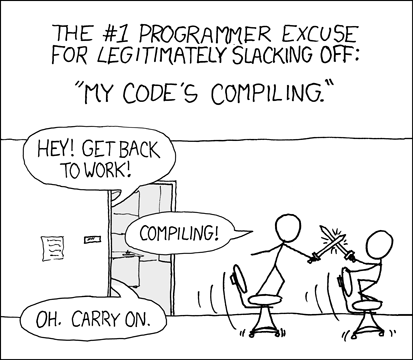
\includegraphics[width=\linewidth]{img/xkcd/compiling.png}
\caption*{{\small \textit{'Are you stealing those LCDs?' 'Yeah, but I'm doing it while my code compiles.' (xkcd/303)}}}
\end{figure}
%Bildlink: http://xkcd.com/303
\addchap{Modulübersicht}

Ein (M) kennzeichnet ein Modul nur für Medieninformatiker, ein (I) jeweils Module für Informatiker und ein (D) für Diplominformatiker.

\minisec{{\Large\ \\ 1. Semester\\\ }}

\textbf{\menu[,]{I, M, D, Einführung in die Mathematik für Informatiker\,}}\\
Du kennst dich mit Matrizen aus?
Dann weißt du auch was mit den Begriffen Determinante, Diagonalisierbarkeit, Skalarprodukt und der Lösung eines homogenen linearen Gleichungssystems anzufangen - wenn nicht, dann lernst du es hier von der Pike an.
Außerdem wird in der Diskreten Mathematik das Mal und Plus quasi neu definiert und du lernst ein wenig anders zu denken.

\textbf{\menu[,]{I, M, D, Algorithmen und Datenstrukturen\,}} \\
Was kommt zuerst?
5 oder 3?
Solche Fragen werden dich in Algorithmen und Datenstrukturen beschäftigen während du Quicksort, Heapsort und Konsorten lernt.
% Der Wortwitz gefällt mir...
Weiter wirst du dich als Gärtner versuchen indem du AVL- und andere Bäume wachsen lasst.
Dabei wirst du Bekanntschaft mit der Programmiersprache C machen.

\textbf{\menu[,]{I, M, D, Einführungspraktikum\,}} \\
Du hast schon immer gerne mit Lego gespielt?
Dann wird dir dieses Praktikum, welches in der vorlesungsfreien Zeit stattfindet, gefallen.
Du darfst dich im Team daran machen einen selbst konstruierten Roboter in C beizubringen, wie er sich in einem Labyrinth alleine zurechtfindet.
Dabei, und im anschließenden Wettbewerb, kommt der Spaß nicht zu knapp.
Für Diplomstudenten gibt es zusätzlich ein einwöchiges Einzelprojekt, bei dem man zeigen kann, was man in C oder wahlweise C++ drauf hat. Alternativ kann das Strategiespielepraktikum auch auf das Sommersemester verschoben werden.
Im letzten Jahr war eine KI für bekannte Brettspiele gefragt.

\textbf{\menu[,]{I, M, Einführung in die Medieninformatik\,}} \\
Anfangs erfolgt eine Darstellung des menschlichen Wahrnehmungssystems, Aspekte der Wahrnehmungspsychologie und der Softwareergonomie.
Dann werden Eigenschaften der Information und Datenformate anhand der Medien Text, Bild, Audio und Video dargestellt.
Im Bereich Text und Bild werden die entsprechenden Dokumentenformate des Internet (HTML und SVG) besprochen.
Ein weiterer Teil der Lehrveranstaltung gibt einen Überblick zur Dokumentenverarbeitung mittels XML-Techniken.
In Übungen und in Form eines Projektes in einer kleinen Gruppe über das Semester hinweg hast du die Möglichkeit, das Erlente direkt in die Praxis umzusetzen.

\textbf{\menu[,]{D, Technische Grundlagen und Hardwarepraktikum\,}} \\
$\rightarrow$ 3. Semester

\textbf{\menu[,]{D, Rechnerarchitektur\,}} \\
$\rightarrow$ 3. Semester


\minisec{{\Large\ \\ 2. Semester\\\ }}

\textbf{\menu[,]{I, M, D, Mathematische Methoden für Informatiker\,}} \\
Nachdem der Abistoff viel tiefer als vorher sitzt, geht es in den nächsten zwei Semestern in neue Bereiche der Mathematik.
Anfangs werden die verschiedenen Typen algebraischer Strukturen (das sind Mengen von beliebigen Symbolen und darauf erklärte Rechenoperationen) untersucht.
Es folgen Vektoren, Matrizen und mathematische Körper.
Dann kommt ein Sprung vom Diskreten zum Kontinuierlichen.
So langweilig wie in der Schule ist Analysis nämlich gar nicht, die gibt es auch in der Ausführung mit mehreren Veränderlichen.
Das Ganze gipfelt in der Einführung von Differentialgleichungen.
Gegen Schluss wendet man sich erneut den Polynomen zu.
Dabei werden zunächst effiziente Näherungsverfahren behandelt.
Später folgt dann ein kurzer Ausflug in die Stochastik.

\textbf{\menu[,]{I, M, D, Programmierung\,}} \\
Dass Programmiersprachen nicht auf Bäumen wachsen, wusstest du wahrscheinlich schon, doch dass sie strengen mathematischen Regeln folgen, lernst du hier.
Am Beispiel eines Teils der Programmiersprache C wird zunächst die Syntax mit Hilfe von Grammatiken definiert.
Kurz darauf kommst du in den Kontakt mit der funktionalen Programmiersprache Haskell.
Durch viele hübsche, rekursiv verschachtelte Abbildungen wird dann die Semantik festgelegt, d.h. die Wirkung, die so ein Programm auf einer (abstrakten) Rechenmaschine hat.
Hier wird auch vermittelt, wie man die Korrektheit eines Programmstückes \glqq wasserdicht\grqq, d.h. formal logisch beweisen kann.

\textbf{\menu[,]{I, M, D, Informations- und Kodierungstheorie\,}} \\
Was Informationen eigentlich sind, was sie ausmacht, wird dich hier beschäftigen.
In dieser Lehrveranstaltung wirst du einen Einstieg in ein sehr interessantes und komplexes Fachgebiet erhalten.
Im Mittelpunkt steht am Anfang wie man Informationen darstellen und speichern kann.
Etwas später wird erklärt, warum und wie die Informationen mittels Kodierung geschützt werden, damit sie bei dir sicher ankommen, wenn sie unterwegs Störungen und Manipulationen ausgesetzt sind.
Dabei wird dir dein in der Mathematik erworbenes Wissen von Nutzen sein.

\textbf{\menu[,]{I, M, D, Softwaretechnologie\,}} \\
Software zu entwickeln ist eine Kunst, das wirst du spätestens nach diesem Modul erkennen.
Um diese Kunstfertigkeit an den Tag legen zu können bedarf es einiger Handwerkszeuge, welche du hier mit auf den Weg bekommst.
So werden dir moderne Konzepte am Beispiel von Java und Entwurfsverfahren zusammen mit professioneller Dokumentation näher gebracht.
Damit wird dann der Grundstein für das Projekt im dritten Semester gelegt, bei dem man sich Lorbeeren im Projektmanagement und als Entwickler verdienen kann.

\textbf{\menu[,]{I, M, Einführung in die Computergraphik\,}} \\
Es geht um den Aufbau von Grafiksystemen, Farbräumen, Rastergraphiken und deren Anwendungen.
Bestehende Probleme, wie Aliasing und Artefakte sind mit von der Partie, sowie ihre algorithmischen Lösungen.
Als Programmiersprache für die Übungsaufgaben wird C++ genutzt.

\textbf{\menu[,]{D, Technische Grundlagen und Hardwarepraktikum\,}} \\
Fortsetzung aus dem 1. Semester.

\textbf{\menu[,]{D, Rechnerarchitektur\,}} \\
Fortsetzung aus dem 1. Semester.


\minisec{{\Large\ \\ 3. Semester\\\ }}

\textbf{\menu[,]{I, M, D, Mathematische Methoden für Informatiker\,}} \\
Fortsetzung aus dem 2. Semester.

\textbf{\menu[,]{I, M, D, Formale Systeme\,}} \\
Wahr?
Und oder falsch?
Was falsch ist wird, wenn es falsch falsch ist, wahr?
Logisch!
Neben der Aussagenlogik vermittelt das Modul die Grundlagen formaler Sprachen.
Es folgen Gedanken zu maschinellen Berechenbarkeit und zur Automatentheorie.
Turing lässt grüßen.

\textbf{\menu[,]{I, M, D, Softwaretechnologie-Projekt\,}} \\
Das Projekt nimmt den größten Teil des dritten Semesters ein.
Hier muss man sein Wissen aus der Lehrveranstaltung \glqq Softwaretechnologie\grqq\ in die Tat umsetzen.
In einem fünfköpfigen Team hast du die Aufgabe, eine Anwendung für einen realen Kunden oder den Lehrstuhl von vorn bis hinten fertig zu stellen.
Dabei muss man häufig Rücksprache mit den Kunden halten.
Abgeschlossen wird das Modul mit einer Präsentation des fertigen Produkts vor dem Kunden und den Verantwortlichen des Moduls.
Am Ende hast du dann einen Eindruck, wie die Arbeit eines Informatikers aussehen kann.

\textbf{\menu[,]{I, M, Rechnerarchitektur\,}} \\
Hier geht es um die Grundbausteine eines Computers:
Speicher, Bussysteme, Rechen- und Steuerwerk.
Außerdem erhält man eine Einführung in Assembler, das Pipelining-Prinzip und damit auftretende Probleme.
Schließlich wird noch diskutiert, mit welchen Methoden man heutige Rechnerarchitekturen beschleunigen kann und parallele Architekturen nutzen kann.

\textbf{\menu[,]{I, Technische Grundlagen und Hardwarepraktikum\,}} \\
Wer schon immer mal wissen wollte, was die Elektronen im häuslichen Rechner eigentlich so alles durchmachen müssen, bekommt das genau vermittelt.
Anfangs werden Transistor-, Dioden- und Operationsverstärkerschaltungen betrachtet.
Darauf aufbauend geht es über Verknüpfungsglieder und komplexe Schaltungen.

\textbf{\menu[,]{M, Grundlagen der Gestaltung\,}} \\
Die Vorlesung beginnt mit Begriffsdefinitionen sowie allgemeinen Gestaltungsprinzipien und erläutert diese.
Dabei beschränkt sich die Veranstaltung bewusst auf zweidimensionale Bereiche.
Formkategorien, Kontrastbildung und Farblehre bilden die Schwerpunkte.
Die begleitenden Übungen sollen einen Einblick in die Materie vermitteln und die Sensibilität der Studierenden durch handwerkliches Arbeiten wecken.

\textbf{\menu[,]{D, Grundlagen des Nebenfachs\,}} \\
Je nachdem, was du dir als Nebenfach wählst, beschäftigst du dich hier mit Themen die nur im entfernten Sinne mit Informatik zusammenhängen.
Über den Tellerrand schauen und andere Welten kennenlernen ist das Motto.

\textbf{\menu[,]{D, Betriebssysteme und Sicherheit\,}} \\
$\rightarrow$ 5. Semester

\begin{figure}[h!]
\centering
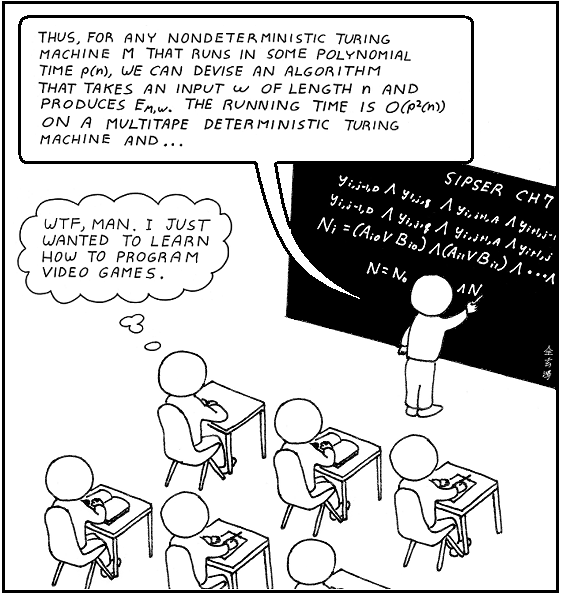
\includegraphics[scale=.5]{img/xkcd/computer_science_major.png}
\caption*{{\small \textit{You'd be surprised how many times the Cook-Levin theorem was used in making the Halo 3 Engine. (http://abstrusegoose.com/206)}}}
\end{figure}

\minisec{{\Large\ \\ 4. Semester\\\ }}

\textbf{\menu[,]{I, D, Theoretische Informatik und Logik\,}} \\
Die Fortsetzung der Formalen Systeme.
Es folgen weitere Betrachtungen zur Korrektheit und Terminierung von Algorithmen und der notwendige Aufwand in Form von Zeit und Platzbedarf.
Ein Abstecher in die Prädikatenlogik und Logikprogrammierung rundet das Modul ab.

\textbf{\menu[,]{I, M, Rechnerarchitektur\,}} \\
Fortsetzung aus dem 3. Semester.

\textbf{\menu[,]{I, M, D, Datenbanken und Rechnernetze\,}} \\
Dies Modul besteht aus zwei verschiedenen Lehrveranstaltungen.
In Datenbanken lernt man zuerst Methoden zur effizienten Datenspeicherung kennen.
Danach wird die Fähigkeit vermittelt, selbst komplexe relationale Datenbanken zu konzipieren und zu erstellen.
In Rechnernetze wird angefangen mit dem Funktionsprinzip von Modem und Netzwerkkarte und man erhält einen kurzen Überblick über moderne Kommunikations- und Vermittlungsprotokolle.
Auch der Sektor Mobilkommunikation und die dabei auftretenden Schwierigkeiten werden kurz beleuchtet.

\textbf{\menu[,]{I, Technische Grundlagen und Hardwarepraktikum\,}} \\
Fortsetzung aus dem 3. Semester.

\textbf{\menu[,]{M, Einführung in die Mediengestaltung\,}} \\
Die Vorlesung vermittelt die Grundzüge des multimedialen Gestaltens unter Gesichtspunkten der Entwicklung der einzelnen Richtungen (Film, Internet) mit Bezug auf die gestalterischen Änderungen in den vergangenen Jahrhunderten (Buch).
Außerdem wird in die Metaphernbildung eingeführt und es werden Schwerpunkte in Richtung des Interfacedesign gesetzt.

\textbf{\menu[,]{M, Medien und Medienströme\,}} \\
Hier wird Wissen zu Medien, deren Kompression und Bearbeitung vermittelt.
Die Anwendung verschiedener Werkzeuge zur Erzeugung von Medien und deren Charakteristika sind ebenfalls Gegenstand dieser Lehrveranstaltung.
So wirst du dich in Form von Übungsaufgaben mit den Grundlagen der Bild-, Audio- und Videobearbeitung auseinandersetzen.

\textbf{\menu[,]{M, Medienpsychologie und -didaktik\,}} \\
Mediendidaktik ist die \glqq Kunst des Lehrens\grqq.
Hier werden die Fragen beantwortet:
Was ist Bildung?
Wie verläuft sie?
Wie lässt sie sich vervollkommnen?
Man erfährt etwas über die Entwicklung von Lehrmethoden.
Im parallel stattfindenden Praktikum wird das Gelernte gleich praktisch bei der Entwicklung eines Lernspiels angewandt.

\textbf{\menu[,]{M, Komplexpraktikum\,}} \\
Das große Highlight für Medieninformatiker im Bachelor.
In kleineren Gruppen soll ein mobiles Spiel, eine Internet-Seite oder Multimediales realisiert werden.
Abgesehen von der Aufgabenstellung sind der Fantasie quasi keine Grenzen gesetzt.
Es geht um harte Arbeit, Teamgeist und das Ernten der wohlverdienten Lorbeeren.

\textbf{\menu[,]{D, Forschungslinie\,}} \\
Hier bekommst du einen Überblick über aktuelle Forschungsthemen und bekommst vermittelt, wie man forschungsorientiert arbeitet.
Dieses Modul hilft, später die richtige Vertiefung zu wählen.

\textbf{\menu[,]{D, Grundlagen des Nebenfachs\,}} \\
Fortsetzung aus dem 3. Semester.

\textbf{\menu[,]{D, Allg. Basisqualifikationen\,}} \\
Englisch ist die einzig relevante Sprache in der Informatik.
Hier wird dir vermittelt, wie man sich fachlich auf Englisch ausdrückt.
Abgerundet wird das Modul durch eine Schulung deiner Vortragsfähigkeiten.


\minisec{{\Large\ \\ 5. Semester\\\ }}

\textbf{\menu[,]{I, M, Betriebssysteme und Sicherheit\,}} \\
Diese Lehrveranstaltung nimmt die dienstbaren Geister, die zwischen der Hardware und den bunten Anwendungen werkeln, unter die Lupe.
Warum kann man mit einem Rechner gleichzeitig einen Text schreiben, Code kompilieren, ein Bild bearbeiten und Musik hören?
Wie werden meine Daten in Rechnersystemen geschützt?
Wieso stehen die hier auf dieses Unix?

\textbf{\menu[,]{I, D, Systemorientierte Informatik/Hardware Software Codesign\,}} \\
Dieses Fachgebiet ist die Schnittstelle zwischen Rechnern und der industriellen Praxis, die von der Steuerung von Heizventilen bis zu Kraftwerken reicht.
Zunächst wird abstrahiert, was allen praktisch vorkommenden Systemen gemein ist, und es werden Modelle wie \glqq System\grqq, \glqq Signal\grqq\ und \glqq Regelkreis\grqq\ erschaffen, mit denen sich dann rechnerisch umgehen lässt.
Hier wird man fit gemacht für die Analyse und Voraussage von Übertragungsverhalten und Reaktionen, die ein solches System bei einem bestimmten Input zeigen wird.
Daneben kommen auch Aspekte aus der Audio- und Videotechnik wie Digitalisierung und Filteralgorithmen nicht zu kurz.

\textbf{\menu[,]{I, D, Intelligente Systeme\,}} \\
In dieser Lehrveranstaltung geht es um künstliche Intelligenz.
Hier erlernt man Problemlösung, Wissensrepräsentation, Planung, Wahrnehmung und Sprachverstehen mit Hilfe spezieller Algorithmen und Agenten.

\textbf{\menu[,]{M, Web- und Multimedia Engineering\,}} \\
Wie kann man das Web mit heutiger Technik multimedial und interaktiv gestalten?
Wie nutze ich professionelle Entwicklungswerkzeuge und geeignete Sprachen, wie z.B. Java, um meine Vorstellung in das Ergebnis zu projizieren?
% professionelle Entwicklungswerkzeuge und geeignete Sprachen (im Bezug auf Webentwicklung) -> Java... Alles klar m(
Dieses Modul hilft geeignete Methoden zu erlernen und Erfahrung bei der Anwendung zu sammeln.

\textbf{\menu[,]{M, Komplexpraktikum\,}} \\
Fortsetzung aus dem 4. Semester.

\textbf{\menu[,]{I, M, D, Vertiefung\,}} \\
Hier kannst du aus einem Angebotskatalog geeignete Veranstaltungen wählen um deinen wissenschaftlichen Horizont zu erweitern.
Die Möglichkeiten umfassen Vorlesungen, Übungen, Praktika, Projektbearbeitungen, Exkursionen, Proseminare, Tutorien und Sprachkurse.

\textbf{\menu[,]{D, Vertiefung im Nebenfach\,}} \\
Nachdem du dir die Grundlagen deines gewählten Nebenfachs angeeignet hast, wird es nun ernst und du steigst tiefer in die Materie ein.

\textbf{\menu[;]{D; Basismodul 1, 2 und 3\,}} \\
Hier wählst du unter sieben verschiedenen Themenkomplexen drei aus und beschäftigst dich mit ihnen.
Zur Wahl stehen Angewandte Informatik, Künstliche Intelligenz, Software- und Web-Engineering, Systemarchitektur, Technische Informatik, Theoretische Informatik und Graphische Datenverarbeitung.
Innerhalb dieser Richtungen stehen euch verschiedene Vorlesungen zur Auswahl.
Für mehr Infos musst du die einschlägigen Webseiten und die Prüfungsordnung lesen.


\minisec{{\Large\ \\ 6. Semester\\\ }}

\textbf{\menu[,]{I, M, Vertiefung zur Bachelorarbeit\,}} \\
Weitere Vertiefung nach gleichem Muster wie im fünften Semester in Vorbereitung auf die Bachelorarbeit.

\textbf{\menu[,]{I, M, Allgemeine Qualifikation\,}} \\
In dieser Art Nebenfach orientierst du dich fächerübergreifend an Themen deines Interesses, um die fachspezifische Kompetenz zu entwickeln.
Auch hier können Veranstaltungen aus einem Katalog gewählt werden.

\textbf{\menu[,]{I, M, Bachelorarbeit und Kolloquium\,}} \\
Als krönenden Abschluss fertigst du die Bachelorarbeit zu einem von dir gewählten Thema an und verteidigst sie in einem Vortrag.

\textbf{\menu[,]{D, Vertiefung im Nebenfach\,}} \\
Fortsetzung aus dem 5. Semester.

\textbf{\menu[;]{D; Basismodul 1, 2 und 3\,}} \\
Fortsetzung aus dem 5. Semester.

\minisec{{\Large\ \\ 7. Semester\\\ }}

Angehende Diplominformatiker haben nach den sechs Semestern noch vier weitere vor sich.
Im siebten Semester wirst du ein Berufspraktikum absolvieren, im achten und neunten wirst du dann Module auswählen die dich interessieren und tiefer in die Abgründe des gewählten Themas hinabsteigen.
Im zehnten Semester wird ausschließlich die Diplomarbeit angefertigt und das war es dann schon!
So schnell kann es gehen.

\vfill

\begin{figure}[h!]
\centering
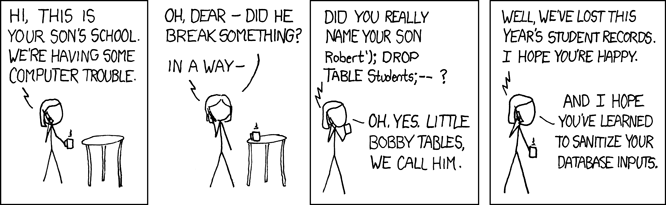
\includegraphics[scale=.5]{img/xkcd/exploits_of_a_mom.png}
\caption*{{\small \textit{Her daughter is named Help I'm trapped in a driver's license factory. (xkcd.com/327)}}}
\end{figure}

\addchap{Press F1 for help}

\minisec{Der Fachschaftsrat}
Nach euren Freunden und Seminargruppenmentoren eure nächste Anlaufstelle.
Wir kümmern uns um eure Probleme oder vermitteln Hilfe.

\minisec{Der Studiendekan}
Neben dem Dekan der Fakultät und seinem Stellvertreter, dem Prodekan, gibt es noch ein weiteres Amt innerhalb der Fakultätsleitung:
den sogenannten Studiendekan.
Er ist für die Angelegenheiten der Lehre in der Fakultät zuständig, bildet den Vermittler zwischen Studenten und Professoren und hilft bei Problemen mit dem Studium allgemein.

Prof. Dr. rer. nat. habil. Weber \\
Büro: APB 1055 \\
Telefon: (0351) 463-38477 \\
E-Mail: gerhard.weber@tu-dresden.de \\

\minisec{Serviceleistung des StuRa}
\begin{itemize}
\item BAföG- und Sozialberatung
\item Rechtsberatung
\item Ausländerberatung
\item Beratung für Studierende mit Kind
\item Beratung zu Anträgen und Förderungsmöglichkeiten
\item Verkauf von Karten für verschiedene Kulturveranstaltungen
\item Material- und Geräteverleih
\end{itemize}

Informationen zu allen Serviceleistungen gibt es im \textit{spiritus rector} und unter \link{\textcolor{red}{NONE}}.
% stura.tu-dresden.de

\minisec{Studienberatung}
Möchtest du dich zu deinem Studiengang beraten lassen oder hast Fragen, dann kannst du dich auch gerne an die Studienberatung wenden.
Studentische Berater sind derzeit Sascha Peukert (Informatik) und Kilian Költzsch (Medieninformatik).
Erreichbar sind sie unter \textit{sascha@ifsr.de} bzw. \textit{koeltzsch@ifsr.de}.
Die Ansprechpartner im Immatrikulationsamt sind auf \link{\textcolor{red}{NONE}} zu finden.
% tu-dresden.de/studium/beratung/studienfachberatung

\minisec{Studium mit Behinderung und chronischer Krankheit}
Unter \link{\textcolor{red}{NONE}} findet ihr Hilfe und Informationen, um mit Handicap im Studium gut zurecht zu kommen.
% tu-dresden.de/die_tu_dresden/gremien_und_beauftragte/beauftragte/bfsb

\minisec{Das Prüfungsamt}
Bei Problemen mit der Prüfungseinschreibung, Notenvergabe oder jeglichen Dingen, die mit deinen Prüfungsleistungen zu tun haben ist das Prüfungsamt der entscheidende Ansprechpartner.

Bei Fristüberschreitungen gelten Prüfungen als nicht bestanden und ihr werdet exmatrikuliert.
Unter Umständen seid ihr aber gar nicht schuld am Verstreichen eines Termins.
Dann müsst ihr einen entsprechenden Antrag an den Prüfungsausschuss (PA) stellen.
Gleiches gilt auch, wenn ihr eine frühere Studienleistung (also einen Leistungsnachweis oder das Ergebnis einer Prüfung) anerkannt haben möchtet.
Vorher solltet ihr unbedingt mit euren zwei studentischen Vertretern im Prüfungsausschuss oder mit dem FSR sprechen.
Die Vorsitzenden der Prüfungsausschüsse sind Prof. Baier (Informatik) und Prof. Groh (Medieninformatik), in dringlichen Fällen könnt ihr euch direkt an sie wenden.

Wo: Prüfungsamt, APB 3039/3040 \\
Wann: Di, Do: 12.30 - 15.00 Uhr \\
Mi: 9.00 - 11.00 Uhr \\
Telefon: (0351) 463-38378

Prüfungsamt-Vorsitzende: \\
Prof. Dr. Christel Baier \\
Büro: APB 3006 \\
Telefon: (0351) 463-38548 \\
E-Mail: christel.baier@tu-dresden.de

Prof. Dr. Rainer Groh \\
Büro: APB 2064 \\
Telefon: (0351) 463-39178 \\
E-Mail: rainer.groh@tu-dresden.de

\begin{figure}[h!]
\centering 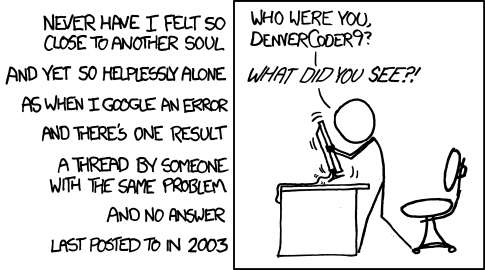
\includegraphics[width=\linewidth]{img/xkcd/wisdom_of_the_ancients.png}
\caption*{{\small \textit{All long help threads should have a sticky globally-editable post at the top saying 'DEAR PEOPLE FROM THE FUTURE: Here's what we've figured out so far ...' (xkcd/979)}}}
\end{figure}
%Bildlink: http://xkcd.com/979

\addchap{auditorium}

\begin{wrapfigure}{l}{5.5cm}

\includegraphics[width=.95\linewidth]{img/auditorium_logo}
\end{wrapfigure}

Wenn du im Internet suchst, findest du nur unübersichtliche Foren?
Wikipedia kann dir auch nicht weiterhelfen?
Deinem Dozenten oder Tutor willst du keine E-Mail schreiben, weil du denkst, dass deine Frage unangebracht ist?

Keine Panik!
Wir haben die Lösung: auditorium.

Mit auditorium bieten wir dir die Möglichkeit, dass du zu den Lehrveranstaltungen Fragen stellen kannst.
Diese können von deinen Kommilitonen oder den Lehrenden beantwortet, kommentiert und bewertet werden.
Wurde eine Antwort, ein Kommentar oder eine Bewertung zu deiner Frage abgegeben, wirst du darüber informiert und kannst direkt nachschauen.

\begin{wrapfigure}{r}{12cm}
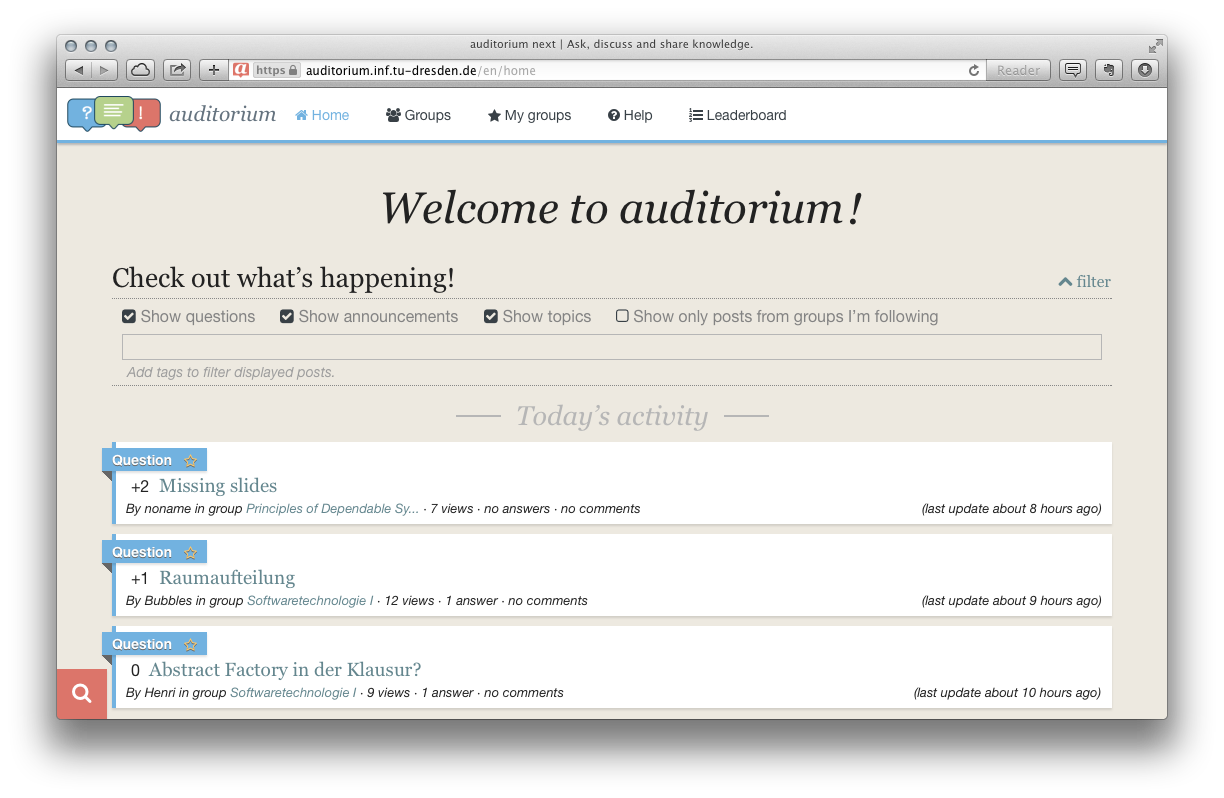
\includegraphics[width=.95\linewidth]{img/auditorium.png}
\end{wrapfigure}

Um immer die wichtigsten Fragen und Neuigkeiten zu erfahren, bietet auditorium die Möglichkeit, Lehrveranstaltungen zu verfolgen.
Folgst du einer Lehrveranstaltung, so bekommst du bei wichtigen Informationen, neuen Fragen oder Antworten eine Nachricht und weißt, was gerade wichtig ist.

Aber als ob das nicht schon hilfreich wäre, entwickeln wir auditorium stets weiter.
Wir haben uns dazu entschlossen den Quellcode auf github.com zur freien Verfügung zu stellen.
Dort kann ihn jeder herunterladen und an der Entwicklung teilnehmen.
Falls du dazu Fragen oder Interesse hast, dann folge uns entweder auf Twitter \textit{@\_auditorium} oder schreibe uns eine Mail an \textit{auditorium@inftex.net}.

\addchap{Der Fachschaftsrat}

\minisec{Wer ist der FSR?}
Der Fachschaftsrat ist eure Vertretung auf Fakultätsebene.
Er wird jährlich gewählt und besteht zur Zeit aus 17 Studenten der Informatik und Medieninformatik.
Als gewähltes Gremium können wir eure Interessen bei den zuständigen Stellen vortragen und so das Studium angenehmer machen.
Neben eurer Vertretung kümmern wir uns um viele weitere Belange.

\minisec{Was wir machen}
Der FSR ist zentrale Anlaufstelle bei Problemen mit dem Studium.
Um es gar nicht so weit kommen zu lassen, unterstützen wir euch im Studium so gut wie es geht.
So sammeln wir alte Prüfungen und Protokolle von Komplexprüfungen und stellen sie für euch online.
Damit die Qualität der Lehre weiter verbessert wird, kümmert sich der FSR um die Evaluation der einzelnen Vorlesungen.
Um euch einen guten Einstieg zu ermöglichen, organisieren wir eine Woche lang und nur für euch die Erstsemestereinführung.

Jedes Jahr gibt es natürlich die obligatorische Weihnachtsfeier.
Wenn es dann wieder wärmer wird, ist es Zeit für die Grillabende oder ein Sportturnier. \\
Außerdem veranstaltet der FSR regelmäßig Spieleabende mit Brett-, Karten- und virtuellen Spielen in der Fakultät.

\minisec{Wir brauchen DICH}
WE WANT YOU TO JOIN THE FSR.
Demokratie lebt vom Mitmachen.
Im Gegensatz zur großen Bundesrepublik ist Demokratie an der Uni direkt, mit niedrigen Hürden verbunden und erfolgreich.
Damit das so bleibt, brauchen wir dich im FSR.
Es kann nur so gut gearbeitet werden, wie motivierte FSRlinge da sind.
Studentenvertretung ist, was ihr daraus macht.

GEH WÄHLEN.
Auch wer sich nicht selbst zur Wahl aufstellen lassen will, kann was für seine Fachschaft tun.
Deine Stimme gibt dem FSR Rückhalt bei schwierigen Entscheidungen.

%TODO: Die PDF ist zu lang...

\includegraphics[width=.5\linewidth]{img/fsr_logo}

Wir suchen auch immer Organisationstalente für einzelne Veranstaltungen wie die Sporttuniere oder die Lange Nacht der Wissenschaften.
Wenn du dich also nicht das ganze Jahr lang offiziell gewählt engagieren willst, kannst du auch als sogenanntes assoziiertes Mitglied jederzeit mithelfen, die Rahmenbedingungen des Studiums an unserer Fakultät zu verbessern.

\minisec{Kontakt}
Jeden Montagabend treffen wir uns um 18:30 Uhr im großen Ratssaal (INF/1004), um unter anderen über verschiedene Aktionen, sei es ESE, Lehrevaluation, Sporttuniere aber auch über Probleme und Entwicklungen an der Fakultät bzw. Universität zu diskutieren und uns zu engagieren.
Ihr seid dabei herzlichst eingeladen, denn die Sitzung ist für alle öffentlich!
Den Rest der Zeit sind wir eigentlich immer im Büro im Erdgeschoss der INF aufzufinden.

Wo: INF/E017 \\
Tel.: (0351) 463-38226 \\
Sitzung: immer montags 18:30 Uhr \\
E-Mail: fsr@ifsr.de \\
Web: www.ifsr.de

\minisec{Dein FSR}


\includegraphics[width=.2\linewidth]{img/fsr/200_jakob_kruse.jpg}

\includegraphics[width=.2\linewidth]{img/fsr/200_robin_trauer.jpg}
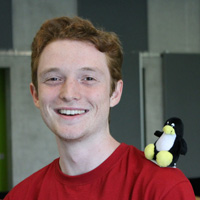
\includegraphics[width=.2\linewidth]{img/fsr/200_kilian_koeltzsch.jpg}

\includegraphics[width=.2\linewidth]{img/fsr/200_philipp_heisig.jpg}

\includegraphics[width=.2\linewidth]{img/fsr/200_simon_hanisch.jpg}

\includegraphics[width=.2\linewidth]{img/fsr/200_tim_hackel.jpg}
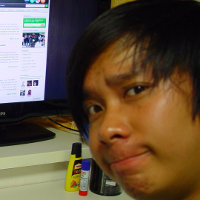
\includegraphics[width=.2\linewidth]{img/fsr/200_duc_nguyen_tien.jpg}

\includegraphics[width=.2\linewidth]{img/fsr/200_sebastian_mielke.png}

\includegraphics[width=.2\linewidth]{img/fsr/200_rico_skultety.jpg}

\includegraphics[width=.2\linewidth]{img/fsr/200_niklas_fallik.jpg}

\includegraphics[width=.2\linewidth]{img/fsr/200_ben_kosmann.jpg}
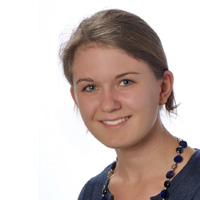
\includegraphics[width=.2\linewidth]{img/fsr/200_katja_linnemann.jpg}
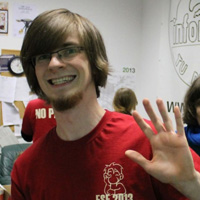
\includegraphics[width=.2\linewidth]{img/fsr/200_marc_satkowski.jpg}

\includegraphics[width=.2\linewidth]{img/fsr/200_anita_gruetzner.jpg}

\includegraphics[width=.2\linewidth]{img/fsr/200_justus_adam.jpg}
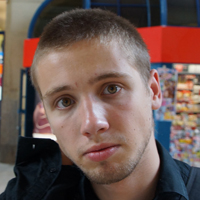
\includegraphics[width=.2\linewidth]{img/fsr/200_manuel_thieme.jpg}

\includegraphics[width=.2\linewidth]{img/fsr/200_sascha_peukert.jpg}

%TODO: Namen und clevere Sprüche zu jedem.
%Wahlweise auch "bekannte" Zitate, weißtebescheid, hier gibt's aber auf jeden Fall doch noch Mitspracherecht des jeweiligen Mitglieds ;)


\newpage
\thispagestyle{empty} %keine Seitenzahl
\AddToShipoutPicture*{\put(0,0){%
\parbox[b][\paperheight]{\paperwidth}{%
\vfill
\centering
\includegraphics[width=\paperwidth,height=\paperheight,%
keepaspectratio]{img/spieleabend.png}%
\vfill
}}}
\mbox{}

\addchap{Studentenclub Count Down}

\begin{wrapfigure}{l}{4cm}%
  \vspace{-.5cm}
  \begin{centering}
    
\includegraphics[width=3.7cm]{img/countdown.jpg}
  \end{centering}%
  \vspace{-.5cm}
\end{wrapfigure}

Um einen Ort für gemeinsame Treffen und Aktivitäten zu haben, betreiben wir vom Studentenklub IZ e.V. das Count Down.
Dieses befindet sich im Keller des Wohnheims Güntzstraße 22 und liegt damit auf halbem Weg zwischen Campus und Neustadt.
Mit einer Mischung aus gemütlichen Kneipenabenden und verschiedenen Parties begleiten wir dein Studentenleben, selbstverständlich zu studentischen Preisen!

Montags findet unser traditioneller und fast schon nostalgischer Spieleabend statt.
Damit es nicht langweilig wird, haben wir eine große Auswahl an verschiedenen Brett- und Kartenspielen parat.

Bei den Erasmus-Partys hast du jeden Dienstag die Gelegenheit, gemeinsam mit ausländischen Studenten zu feiern und deren Kulturen kennen zu lernen.

Darüber hinaus gibt es auch viele Veranstaltungen, die nicht im festgeschriebenen Rhythmus stehen, aber trotzdem immer wieder stattfinden.
Dazu gehören unter anderem ein Kneipenquiz, Cocktail- und Bowleabende, sowie der Metalalterabend.
Den aktuellen Plan findest du auf unserer Internetseite: \url{countdown-dresden.de}.

Du willst gern einmal selbst auf der Bühne stehen?
Ob mit der Blockflöte oder einem spannenden Reisebericht:
Auch dafür ist bei uns Platz im Klub und Kalender!

Und solltest du keine fremden Zuschauer haben wollen, sondern einfach mit deinen Freunden eine Party außerhalb deiner eigenen vier Wände geben, bist du ebenfalls bei uns genau richtig.
An allen Tagen, an denen wir keine Veranstaltung geplant haben (insbesondere am Freitag und Samstag), hast du die Möglichkeit, unseren Klub zu studentisch günstigen Preisen zu mieten, Barpersonal, Aufräumen und Putzen inklusive.
Schau einfach auf unsere Homepage und reservier' einen Termin!

Das reicht dir immer noch nicht?
Du möchtest das Studentenleben gern selbst mit gestalten?
Du triffst gerne viele neue, nette Leute?
Du hast vielleicht sogar weitere Ideen für interessante Veranstaltungen?
Du möchtest gern einmal selbst an der Bar stehen und dabei nicht den Chef im Nacken sitzen, sondern den Spaß im Vordergrund stehen haben?
Sprich uns einfach direkt an, neue Mitglieder sind immer herzlich willkommen.

Ob als Gast oder als neues Mitglied - wir freuen uns, dich bald bei uns begrüßen zu dürfen.

\textit{Dein Team vom Count Down}

\addchap{ASCII - Das Café in der Fakultät}

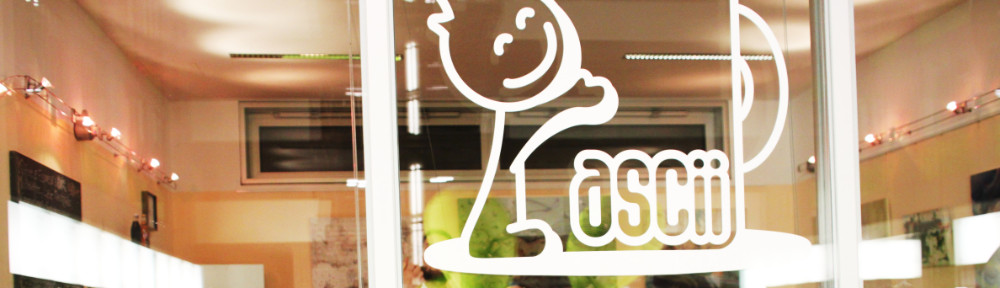
\includegraphics[width=\linewidth]{img/ascii.jpg}

Seit 2007 gibt es in der Fakultät Informatik das ASCII, ein von Studenten betriebenes Café ganz nach der Vorstellung eines richtigen Informatikers.
Es gibt neben diversen Kaffeesorten auch kalte Getränke (Stichwort Mate) und sogar Bagels, Muffins und Donuts, sprich:
alles was ein müder Informatiker morgens braucht, wobei \glqq morgens\grqq\ auch gerne mal 13 Uhr sein kann.
Das ASCII zählt zudem zu den wenigen Adressen auf dem Campus, in denen man Kolle Mate, Club Mate und Premium Cola erhält.
Hinter dem Tresen stehen fast ausschließlich Studenten, die an einem Tag in der Woche noch ein paar Stündchen zur Verfügung stellen können.
Das heißt es werden auch jedes Semester neue Leute gesucht, die gerne mitmachen wollen.

Das ASCII ist seit seiner Gründung zu einer zentralen Anlaufstelle an unserer Fakultät geworden.
Hier treffen sich Studenten, Mitarbeiter und Professoren der Informatik, aber auch Besucher von anderen Fakultäten kommen gerne vorbei um hier ihre Kaffeepausen zu verbringen oder ihren Koffeinhaushalt aufzufüllen.
Auf den gemütlichen Sofas kann man die Zeit wunderbar an sich vorbei streichen lassen, gemeinsam an Projekten arbeiten, lernen, programmieren oder einfach nur mit seinen Kommilitonen plaudern.
Wenn du jetzt Lust bekommen hast, das ASCII auch mal zu besuchen oder sogar als Mitglied selbst hinter dem Tresen zu stehen, dann komm doch einfach mal vorbei und sag hallo!

Das aktuelle Angebot oder Aktuelles erreicht ihr unter \link{http://www.ascii-dresden.de/}.

\textit{Wir öffnen in der Vorlesungszeit Montag bis Donnerstag von 9 bis 17 Uhr und Freitags von 9 bis 15 Uhr.}

\addchap{ZIH}

%TODO: lustige Bildchen/Cliparts (höhö) um alles aufzulockern?

Das \textit{Zentrum für Informationsdienste und Hochleistungsrechnen} ist eine zentrale Einrichtung nicht nur unserer Fakultät, sondern der gesamten TU Dresden und ist für die gesamte Serverinfrastruktur und diverse technische Dienste verantwortlich. Vom ZIH werden dir ein paar sehr hilfreiche und relevante Dienste bereitgestellt, u.a. gehören dazu dein Login, dein E-Mail Account und das WiFi auf dem Campus.

Detailreiche Informationen zu den Services und deren Nutzung findest du auf dem ZIH Flyer, den du mit deinem Immatrikulationsbogen erhalten hast und auf der Seite des ZIH.
%\url{tu-dresden.de/zih/ese}. Wie genau machen wir das jetzt eigentlich mit den Links? Fortlaufende Nummern, die dann auf einer Linkseite hinten und/oder per Shortlink über unsere Seite irgendwie zugänglich sind? Beides zusammen wäre sicher nicht falsch.

\minisec{E-Mail}
Du bekommst vom ZIH zwei E-Mail Adressen:
\textit{s1234567@mail.zih.tu-dresden.de} und einen Alias von der Form \textit{vorname.nachname@mailbox.tu-dresden.de}.
Falls dein Name an der TU Dresden bereits existiert, lautet die Alias-Adresse für Max Mustermann dann z.B. \textit{max.mustermann1@mailbox...}.
Per Webmail oder IMAP kannst du auf dein Postfach zugreifen.
Alternativ kannst du deine Mails an eine persönliche Adresse weiterleiten, damit du nichts verpasst.
Vor allem wichtige E-Mails von der Uni werden an diese Adressen geschickt.

\minisec{WLAN}
Sowohl auf dem Campus wie auch in den Räumlichkeiten der Fakultät kannst du mit deinen Geräten ins Internet.
Das Netzwerk heißt \textit{eduroam} und bietet dir neben einem sicheren Internetzugang an unserer Uni selbes auch an sehr vielen anderen Universitäten weltweit. 
Zugang bekommst du mit deinem Login \textit{sXXXXXXX@tu-dresden.de} und deinem Passwort. Mehr Informationen findest du unter \link{NONE}.

\begin{figure}[h!]
\centering 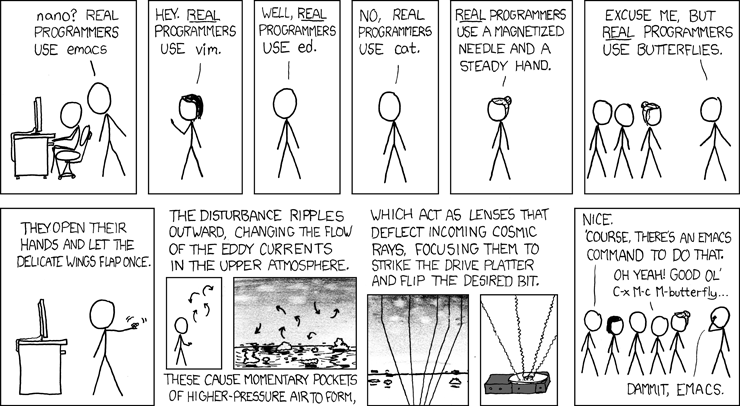
\includegraphics[width=\linewidth]{img/xkcd/real_programmers.png}
\caption*{{\small \textit{Real programmers set the universal constants at the start such that the universe evolves to contain the disk with the data they want. (xkcd/378)}}}
\end{figure}
%Bildlink: http://xkcd.com/378

\twocolumn

\addchap{Glossar}

\textbf{AG DSN} \\
Die AG Dresdner Studentennetz kümmert sich um das Internet in einigen Wohnheimen.
Mithelfer werden laufend gesucht.

\textbf{Anmelden} \\
Alle, die in Dresden heimisch geworden sind, sollten nicht vergessen, sich beim Ortsamt des jeweiligen Stadtbezirkes innerhalb von zwei Wochen anzumelden.

\textbf{APB} \\
Steht für Andreas-Pfitzmann-Bau und ist seit Mitte 2014 offiziell der Name der Fakultät Informatik, deren Kürzel vorher INF war. Ihr werdet sicherlich auf beide Kürzel stoßen, die Änderung ist noch sehr frisch.

\textbf{AQuA} \\
Abkürzung für Allgemeine Qualifikation.
Ist ein Bestandteil deines Studiums.
Genaueres:
Siehe Prüfungs- und Studienordnung.

\textbf{Assistent} \\
Wissenschaftlicher Mitarbeiter am Lehrstuhl, meist Doktor.
Leitet oft Übungen oder Seminare.

\textbf{Auslandsstudium} \\
Etwas, das sich im Lebenslauf immer ganz gut macht, von der Erfahrung und möglicherweise guten Bräune ganz abgesehen.
Nähere Informationen gibt es entweder bei uns im FSR oder im Akademischen Auslandsamt.

\textbf{Bachelor} \\
Die neuen bundesweit eingeführten Abschlüsse.
Merkmale sind ein im Vergleich zum Diplom kürzeres Studium und die Möglichkeit, aufbauend einen Master zu erwerben.

\textbf{BAföG} \\
Zum Thema BAföG gibt es sowohl beim StuRa als auch im Studentenwerk Infomaterial und Anträge.
Beantragt wird BAföG beim BAföG-Amt im Studentenwerk, Fritz-Löffler-Str. 18.
Kümmere dich so schnell wie möglich darum, da frühestens ab dem Antragsmonat gezahlt wird.

\textbf{Belegen} \\
Das Hören einer Vorlesung wird auch als Belegen bezeichnet.
Die im Semester gehörten Vorlesungen müssen in den Belegbogen auf der Rückseite des Studienbuchblattes, das dir mit dem Studentenausweis zugeschickt wurde, eingetragen werden.
Dieses solltest du im Studienbuch abheften.
% macht das überhaupt irgendwer? :D

\textbf{Beurlaubung} \\
Auf Antrag gewährt die Uni zwei freie Urlaubssemester.
Nutz diese Möglichkeit, falls du mal ein Semester frei nehmen willst/musst, damit dir dieses Semester nicht als Fachsemester angerechnet wird.
Achte jedoch auf Bestimmungen zur Höchststudiendauer vor allem zum BAföG.

\textbf{Bibliothek} \\
Primär von Interesse ist für dich die Universitätsbibliothek (SLUB), die du kostenlos nutzen kannst.
Abgesehen davon stehen dir natürlich auch die städtischen Bibliotheken Dresdens zu Verfügung.
Allerdings gibt es für diese eine Jahresgebühr von 12 EUR.

\textbf{Bücher} \\
Es ist ratsam, nicht direkt zum ersten Semester einen Stapel Bücher zu kaufen.
Besser ist es, sich bei höheren Semestern vorher zu erkundigen, welche Literatur ratsam ist.
Außerdem sollte man sich die Bücher, die von Professoren vorgeschlagen werden, zunächst erstmal in der Bibliothek anschauen.
Angebote für gebrauchte Bücher findest du unter anderem in den Campuszeitungen.

\textbf{Campus} \\
Kerngelände der Uni.

\textbf{Campuszeitung} \\
Die zwei Dresdner Campuszeitungen \textit{ad-rem} und \textit{CAZ} erscheinen ein- bzw. zweiwöchentlich.

\textbf{Club Mate} \\
Das ultimative Kultgetränk unter Hackern dieser Welt und im ASCII erhältlich.
Positiver Nebeneffekt nach dem Genuss von Club Mate ist, dass der hohe Koffeingehalt munter macht/hält.
(Nicht mehr ganz so Geheim-)Tipp:
Auch mal die Dresdner Kolle-Mate im ASCII probieren.

\textbf{Creditpoints} \\
Sammelst du mit dem Bestehen von Modulen.
Die Anzahl gibt an wieviel Zeit du aufgewendet hast, bzw. haben sollst.

\textbf{DAAD (Deutscher Akademischer Austauschdienst)} \\
Deutschlandweite Anlaufstelle für das Auslandsstudium.

\textbf{Dekan} \\
Der Dekan leitet und vertritt die Fakultät und führt die Beschlüsse des Fakultätsrates aus.
Der gegenwärtige Dekan ist Prof. Baader.

\textbf{dies academicus} \\
Am "akademischen Tag" finden anstelle der Vorlesungen und Übungen andere Veranstaltungen statt.
Er dient dazu, den Studenten die Möglichkeit zu geben, einmal einen Blick in andere Fachbereiche zu werfen.

\textbf{Diplom} \\
Alternativer Studienabschluss zum Bachelor.
Im Wintersemester 2010 wurde ein neuer, modularisierter Diplomstudiengang (nur Informatik und Informationssystemtechnik) an unserer Fakultät eingeführt.
Im Gegensatz zum Bachelor bietet dieser ein Nebenfach und ein Praktikumssemester.
Das Diplom berechtigt wie ein Master zur Promotion zum Doktor.

\textbf{DrePunct} \\
Bibliothek am Zelleschen Weg 17 (gegenüber der SLUB), die unter anderem die Bücher des Fachbereichs Informatik beinhaltet.

\textbf{Emeal} \\
Der Emeal (auch Mensakarte) wird gebraucht, um in den meisten Mensen Essen zu bekommen.
Er ist gegen eine Kaution von 5 EUR und Vorlage der Emeal-Bescheinigung sowie des Personalausweises an den Kassen der Mensen erhältlich.
Zu Beginn des jeweils nächsten Semesters muss der Emeal verlängert werden.
Im Rahmen der ESE wird die Mensakarte aber auch direkt ausgeteilt.

\textbf{Erasmus} \\
Eine europaweite Initiative zum Studentenaustausch.
Siehe auch Auslandsstudium.

\textbf{EVA} \\
Lehrevaluation, gegen Ende des Semesters füllst du in jeder Vorlesung einen Fragebogen aus, um den Dozenten, die Vorlesung und die Übungsleiter zu bewerten.

\textbf{Exmatrikulation} \\
Beim Austritt aus der Hochschule (Studienende/-abbruch, Wechsel der Hochschule) muss man sich exmatrikulieren.
Zwangsweise geschieht dies, wenn man die Höchststudiendauer überschreitet oder vergisst, sich rückzumelden oder notwendige Prüfungen endgültig nicht bestanden hat.

\textbf{Fachschaft} \\
Alle Studenten einer Fakultät. Also auch du.

\textbf{Fachschaftsrat} \\
Gewählte studentische Vertreter einer Fachschaft.
Deine studentischen Vertreter findest du im Raum E017.
Der Fachschaftsrat freut sich auch immer über Studenten, die mal vorbeischauen und über Probleme oder Anregungen berichten.

\textbf{Fachschaftsratsitzung} \\
Findet einmal wöchentlich im Fachschaftsrat statt.
Hier werden Aktionen geplant, Angelegenheiten der Fakultät diskutiert und vieles mehr.
Jeder ist dazu herzlich eingeladen!
Termine und Sitzungsprotokolle gibt es auf der FSR-Homepage.
Derzeit:
Jeden Montag 18.30 Uhr im großen Ratssaal (APB/1004).

\textbf{Fakultät} \\
In Fakultäten werden verschiedene Fachrichtungen zu einer Lehr- und Verwaltungseinheit zusammengeschlossen (z.B. Fakultät Informatik, Philosophische Fakultät, etc.).

\textbf{FRZ (ZIH)} \\
Das Rechenzentrum in der Informatikfakultät wurde früher von dieser betrieben.
Heute gehört es mit zum ZIH.
Der Rechnerpool bietet dir Gelegenheit, deine Projekte innerhalb der Fakultät zu bearbeiten.
Vorlesungsskripte und Übungsaufgaben einsehen und ausdrucken gehört zu den häufigeren Nutzungen der Rechner.

\textbf{Hochschulsport} \\
Siehe USZ.

\textbf{Immatrikulationsamt} \\
Zuständig für Aktivitäten wie Immatrikulation, Exmatrikulation und Rückmeldung.
Zu finden im Bürohaus Strehlenerstr. 24, 6. Etage und im Netz \link{http://tu-dresden.de/imma/}.

\textbf{I'm So Meta Even This Acronym}
%oh yeah

\textbf{INF} \\
siehe APB.

\textbf{Integrale} \\
Kommentiertes Vorlesungsverzeichnis, in dem alle studium generale Veranstaltungen zu finden sind.

\textbf{jExam} \\
Online-Plattform für Studenten.
Hier kannst du dich für Übungen, Seminare, Praktika, Prüfungen, etc. einschreiben und deine Prüfungsergebnisse abrufen.
Zur Einschreibung in der ESE Woche richtest du deinen Account ein und wir zeigen dir direkt, wie du dich einschreiben kannst.

\textbf{Kino} \\
In Dresden gibt es mehrere Kinos, sowohl wahre Paläste für die unbeschwerte Popcornunterhaltung, als auch kleinere Programmkinos wie beispielsweise das Kino in der Fabrik und Thalia.
Es sei hier auf den spiritus rector verwiesen, in dem alle Kinos aufgeführt sind.

\textbf{Klausur} \\
Schriftliche Prüfung zu einer Vorlesung, meist am Ende des Semesters.
Auf der Seite des FSR sind viele Klausuren vergangener Jahre erhältlich (dieses Archiv ist nur aus dem Uninetz erreichbar).

\textbf{Kopieren} \\
An vielen Stellen der Uni stehen Kopierer.
Um sie zu benutzen, braucht man eine Kopierkarte.
Die Karten der Firma Ricoh sind im StuRa (Zimmer 1 bzw. 4) und an verschiedenen Kartenautomaten, die über den Campus verteilt sind, gegen einen Pfand von 5 EUR erhältlich.
Will man mit den Karten auch drucken, sollte man dies vorher angeben.
Bei Bedarf lässt sich diese dann an den entsprechenden Automaten aufladen.
Eine Kopie kostet 5 Cent.
Zusätzlich hast du die Möglichkeit, im Büro des FSR zu kopieren.
Zu guter Letzt hat auch die SLUB ein von der Firma Acribit betriebenes Kopier-/Drucksystem, natürlich auch mit einer eigenen Karte.
Außerdem gibt es auf dem Campus verteilt noch etliche Copyshops.

\textbf{Krankenversicherung} \\
Ab dem 25. Lebensjahr musst du eine eigene abschließen, bis dahin bist du meist über die Familienversicherung deiner Eltern mit abgesichert.
Informiere dich bestenfalls direkt bei deiner Krankenkasse zu diesem Thema.

\textbf{Kryptografie} \\
Mathe, die deine Kommunikation beschützt.
Such' mal nach GnuPG, signiert und verschlüsselt deine E-Mails.

\textbf{Leistungsnachweis, Schein} \\
Muss in einigen Fächern erbracht werden, um zu bestimmten Prüfungen zugelassen zu werden.
Im Gegensatz zu den Prüfungen ist er beliebig oft wiederholbar und meist unbenotet.
Das ist jedoch kein Freibrief zum Durchfallen, da man die Scheine für Klausuren oder die Bachelorprüfung benötigt.

\textbf{LSK} \\
Lehrzentrum Sprachen und Kulturen, s. Seite \pageref{sec:sprachausbildung}.

\textbf{Matrikelnummer} \\
Die Nummer, unter der du an der Uni als Student geführt wirst.
Steht auf deinem Studentenausweis.
Du brauchst sie z.B. bei Klausuren und Prüfungen.
Es ist deswegen günstig, sie auswendig zu wissen bzw. den Studentenausweis immer dabei zu haben.
Letzteres lohnt sich sowieso, da er auch dein Semesterticket ist.
Matrikelnummer bitte nicht mit der s-Nummer verwechseln.

\textbf{Mensa} \\
Es gibt mehrere Mensen auf dem Campus und an den verschiedenen ausgelagerten Fakultäten.
Im Zuge der allgemeinen Technisierung ist in der Mensa ein bargeldloses Zahlungssystem (Emeal) eingeführt worden.
Wo sich welche Mensa befindet und was es an bestimmten Tagen dort Leckeres zu Essen gibt, kann man auf der Seite des Studentenwerkes in Erfahrung bringen.
Für Smartphones gibt es auch etliche mobile Apps.

\textbf{N.N. (nomen nominandus)} \\
Zu Deutsch:
"(noch) zu nennender Name".
Bedeutet:
der Dozent steht noch nicht fest.

\textbf{No Panic} \\
Dieses Heft.
Ein Eigenname aus historischen Gründen und kein falsches Englisch.

\textbf{Prüfungen} \\
Irgendwann muss da jeder ran.
Hierüber sollte man sich genauestens in der Prüfungsordnung informieren.
Prüfungen können nur begrenzt wiederholt werden.
Wichtig ist natürlich auch die Anmeldung zur Prüfung, diese auf keinen Fall vergessen!
Auch daran denken zu jeder Prüfung den Perso und den Studentenausweis dabei haben!
Prüfungen zu schieben ist auch nur eine begrenzt gute Idee, das holt einen schnell wieder ein.

\textbf{Prüfungsamt} \\
Um zu bestimmten Prüfungen zugelassen zu werden, muss man sich beim Prüfungsamt dazu anmelden.
Eventuell muss man auch Scheine, die für die jeweilige Prüfung Voraussetzung sind, vorzeigen.
Weiterhin kann man hier auch Prüfungsergebnisse erfahren und sich für's Nebenfach einschreiben.

\textbf{Prüfungsordnung} \\
Dort erfährst du, welche Prüfungen und Leistungsnachweise für die Bachelorprüfung benötigt werden und welche Fristen einzuhalten sind.
Diese sollte unbedingt gelesen werden, damit man zumindest weiß, warum man irgendwann plötzlich exmatrikuliert wurde.

\textbf{Prüfungszeit} \\
In den Wochen nach den Vorlesungen wirst du wahrhaftig geprüft.
Prüfungen sollten sechs Wochen vor der Prüfungsperiode im Termin feststehen.
Zu einer Prüfung muss man sich per jExam anmelden.
Abmeldungen (Rücktritte) sind unter bestimmten Voraussetzungen ebenfalls über jExam möglich.

\textbf{Rechtsberatung} \\
Eine kostenlose Rechtsberatung bietet dir der StuRa (Do 13-14 Uhr, 14-tägig) und der Justiziar des Studentenwerkes.
% stimmt noch

\textbf{Rektor} \\
Leitet und vertritt die Universität.
Derzeit Prof. Hans Müller-Steinhagen.

\textbf{Rekursion} \\
Siehe Rekursion.

\textbf{Rückmeldung} \\
Jeder Student, der im darauffolgenden Semester weiter an der Uni studieren möchte, muss sich im angegeben Zeitraum rückmelden.
Die Rückmeldung erfolgt durch fristgemäßes Überweisen des Semesterbeitrags.
Das Formular dafür befindet sich auch immer auf dem Semesterbogen.
Die Höhe des Semesterbeitrags wird auf den Webseiten des Immatrikulationsamts bekanntgegeben.

\textbf{Rundfunkgebühren} \\
Studenten, die nicht zu Hause wohnen, müssen ihren Haushalt anmelden.
Für manche Studenten (z.B. BAföG-Empfänger) besteht jedoch die Möglichkeit, sich von der Gebührenpflicht befreien zu lassen.
Dies ist direkt bei der Rundfunkzentrale zu beantragen.
Bedenke auch, dass du rückwirkend mit deinem Einzugsdatum zur Kasse gebeten werden kannst, eine verspätete Anmeldung bringt also keinen Vorteil.

\textbf{Schein} \\
Siehe Leistungsnachweis.

\textbf{Semesterticket} \\
Wird automatisch mit der Überweisung des Semesterbeitrags bezahlt.
Dein Studentenausweis in Verbindung mit einem gültigen Personalausweis gilt als Fahrschein und ist nicht übertragbar.
Dein Semesterticket gilt auch für den Regionalbahnverkehr in ganz Sachsen.

\textbf{SHKs} \\
Studentische Hilfskräfte werden von den Lehrstühlen als Tutoren oder für wissenschaftliche Hilfstätigkeiten eingestellt.

\textbf{Skript} \\
Oft veröffentlicht der Dozent einer Vorlesung ein eigenes Skript, das dann im Netz öffentlich zugänglich ist und ausgedruckt werden kann.
Diese Skripte sind jedoch nur als Gerüst einer Vorlesung anzusehen und reichen nicht für ein selbständiges Eigenstudium aus.
Damit wollen die Professoren verhindern, dass niemand mehr in den Vorlesungen auftaucht.

\textbf{SLUB} \\
Das Hauptgebäude der Sächsischen Landes-, Staats- und Universitätsbibliothek befindet sich am Zelleschen Weg 18 und ist nicht nur wegen seines schönen, ruhigen Lesesaals immer einen Besuch wert.
Dazu gibt es einige Zweigstellen wie den DrePunct.
Zum Ausleihen von Büchern benötigst du einen Bibliothekausweis, den man jederzeit in der Hauptbibliothek beantragen kann.

\textbf{spiritus rector} \\
Der \glqq leitende Geist\grqq , ein unentbehrliches Heftchen, jedes Jahr von einigen Enthusiasten im StuRa hergestellt.
In ihm kann man u.a. sämtliche Adressen von Kneipen oder Fachschaftsräten finden.
Erältlich beim FSR oder direkt beim StuRa.

\textbf{STAV} \\
Die studentische Arbeitsvermittlung bietet eine Liste von aktuellen Jobs an.
Findet man in der StuRa-Baracke oder auf deren Webseite.

\textbf{Studentenrat (StuRa)} \\
Er vertritt die studentischen Interessen gegenüber der Universität und der Politik und kümmert sich unter anderem um die Verhandlung deines Semestertickets oder um gravierende Probleme mit dem Studentenwerk oder anderen Institutionen.
Außerdem bietet er auch Beratung bei studienrelevanten Problemen (BAföG, etc.) an.
In der StuRa-Baracke befinden sich neben dem Servicebüro des StuRas auch die Büros von STAV und Integrale.

\textbf{Studentenwerk} \\
Fritz-Löffler-Str. 18.
Das Studentenwerk ist zuständig für die Mensen, Studentenwohnheime, BAföG, Beratungen, Wohnungsvermittlung, etc.

\textbf{Studienbuch} \\
In das Studienbuch musst du deine ausgefüllten Studienbuchblätter zusammen mit erlangten Scheinen abheften.

\textbf{Studienordnung} \\
Die Studienordnung legt einen Rahmen für den Ablauf eines Studiums fest, z.B. welche Vorlesungen gehört werden sollten.
Studienordnungen kannst du beim Prüfungsamt, der Studienberatung oder beim FSR bekommen.
Außerdem solltest du im Laufe der ESE zusammen mit dieser No Panic eine erhalten haben.
Unbedingt mal lesen, denn sie enthält deine Rechte und Pflichten.

\textbf{studium generale} \\
Freiwilliges Vorlesungsangebot zum über-den-Tellerrand-schauen.
Siehe Integrale.

\textbf{SWS (Semesterwochenstunden)} \\
Die SWS sind eine Maßeinheit für die Menge von Vorlesungsstunden, die man pro Semester von einer spezifischen Vorlesung besuchen muss.
2 Semesterwochenstunden entsprechen 90 Minuten pro Woche in der Vorlesungszeit.
Wenn man z.B. im zweiten Semester 3 SWS Mathevorlesungen besuchen muss, heißt das, dass man in jeder Woche eine Doppelstunde und zusätzlich alle 2 Wochen noch einmal eine Doppelstunde Mathe zu hören hat.
Durchschnittlich gibt das 3 SWS Vorlesungen in jeder Woche.

\textbf{TUDIAS} \\
TUD Institute of Advanced Studies, s. Seite \pageref{sec:sprachausbildung}.

\textbf{Übungen} \\
Hier wird der Vorlesungsstoff praktiziert.
Es wird von dir als Student erwartet, das Übungsblatt vorher zumindest anzuschauen, um dann die Lösungen zu diskutieren.

\textbf{USZ (Universitätssportzentrum)} \\
Die Universität bietet eine breite Palette von Sportarten zu günstigen Preisen an (normalerweise 15 EUR pro Semester).
Welche Sportarten angeboten werden und wie du dich anmeldest, kannst du auf der Webseite oder im Hochschulsportprospekt, der ab Semesterbeginn überall ausliegt, nachlesen.
Zum Semesterbeginn findet die Einschreibung online statt.
Auf die Termine dafür unbedingt achten, beliebte Kurse sind sehr schnell voll!

\textbf{VL} \\
Vorlesung

\textbf{Wahlen} \\
Gibt es immer im Wintersemester für die Fachschaftsräte der Fakultäten der Uni, die dann Vertreter in den StuRa und in die verschiedenen Gremien entsenden.
Weiterhin können die studentischen Mitglieder des Fakultätsrates gewählt werden.

\textbf{xkcd} \\
Informatiker-Kult-Webcomic auf \url{xkcd.com}. Du findest einige xkcd-Comics in diesem Heft - aber als Informatiker solltest du natürlich alle kennen ;)

\textbf{ZIH} \\
Das Zentrum für Informations- und Hochleistungsrechnen.
Es ist zuständig für alles was mit Computern, Logins, E-Mail, WiFi usw. zu tun hat.

\onecolumn

\addchap{Links}

Alle Links sind auch direkt als \url{ese.ifsr.de/2020/<Zahl>} aufrufbar.

{%
\small
\begin{longtable}{r p{11cm}}
\linklist%
\end{longtable}
}


\addchap[Campusplan]{}
\thispagestyle{empty} %keine Seitenzahl
\AddToShipoutPicture*{\put(0,0){%
\parbox[b][\paperheight]{\paperwidth}{%
\vfill
\centering
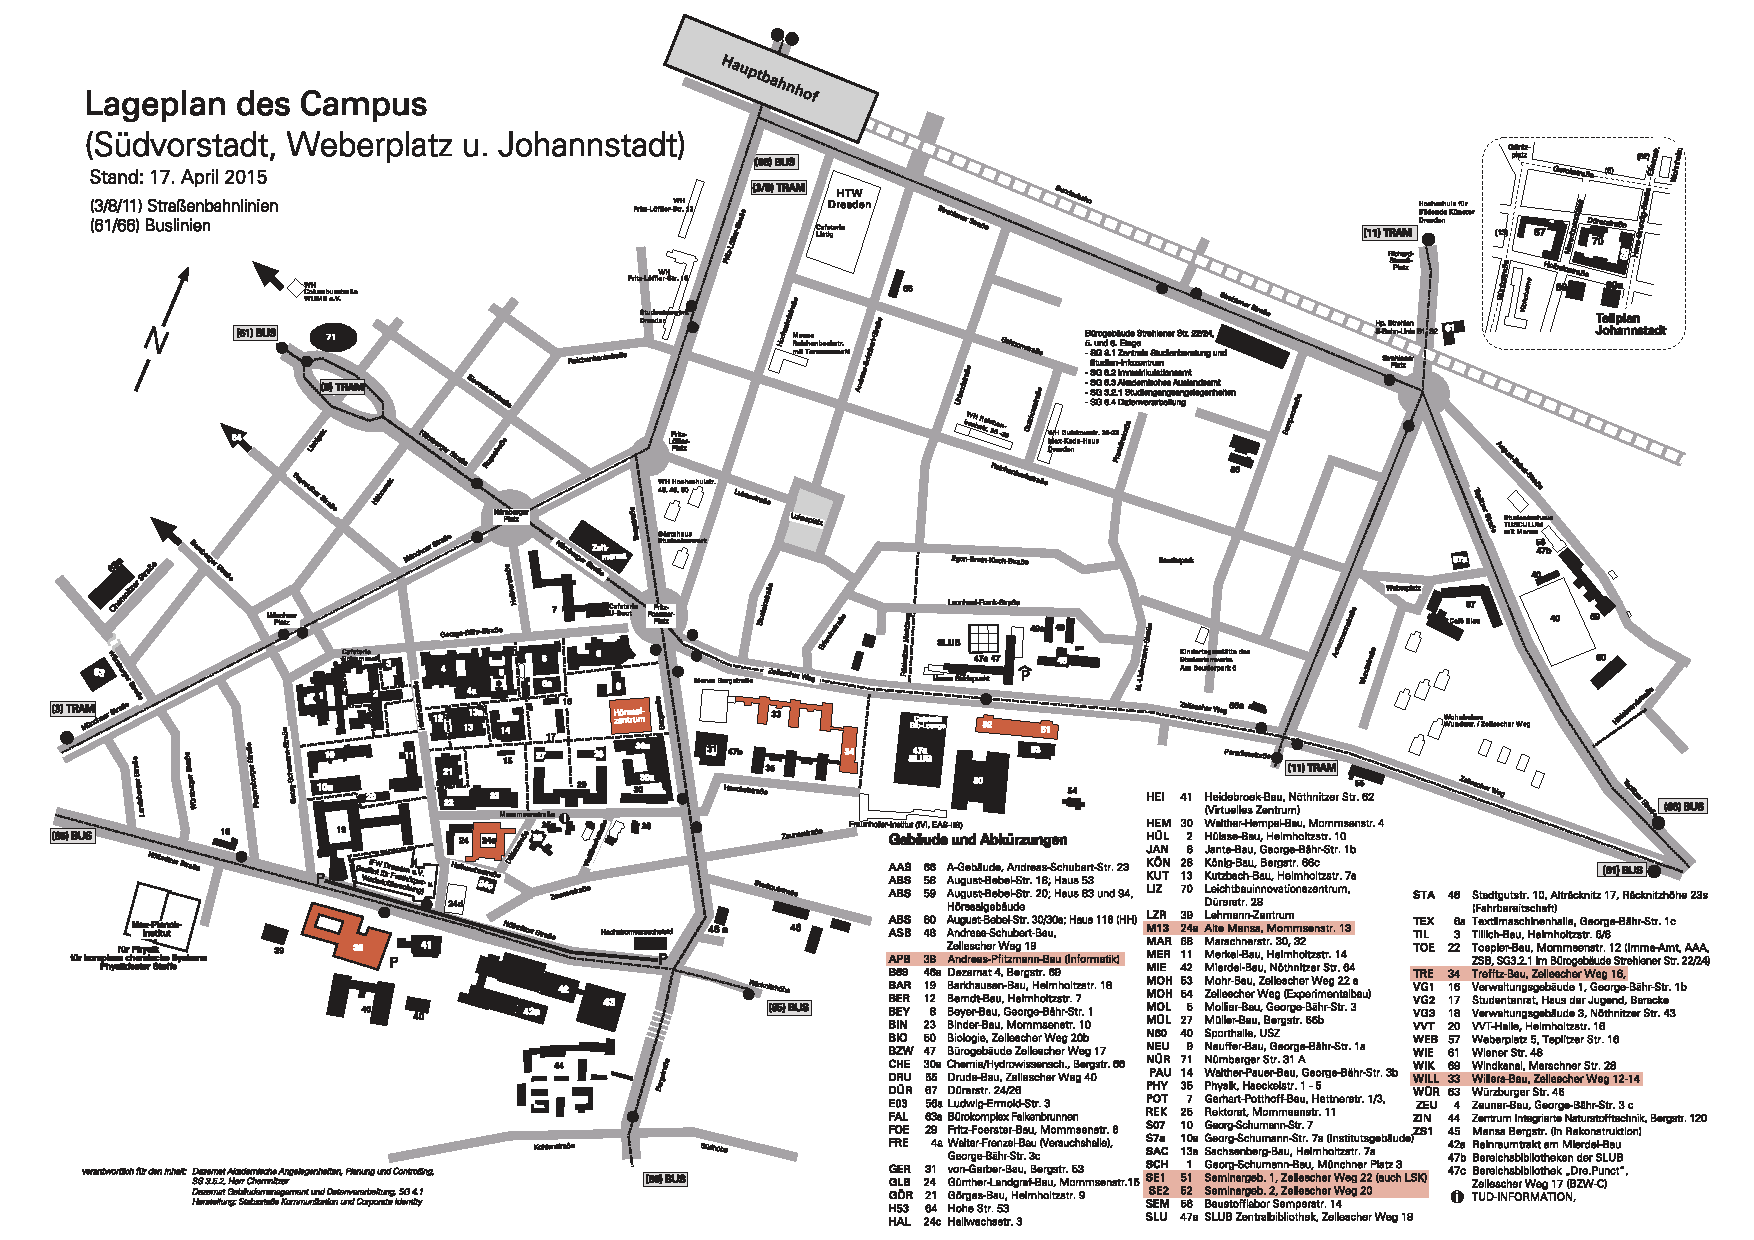
\includegraphics[width=\dimen107,height=\dimen108,keepaspectratio,trim=0 0 1.003\dimen107 0,clip]{img/campusplan_highlighted.pdf}%
\vfill
}}}
\mbox{}
\newpage
\thispagestyle{empty} %keine Seitenzahl
\AddToShipoutPicture*{\put(0,0){%
\parbox[b][\paperheight]{\paperwidth}{%
\vfill
\centering
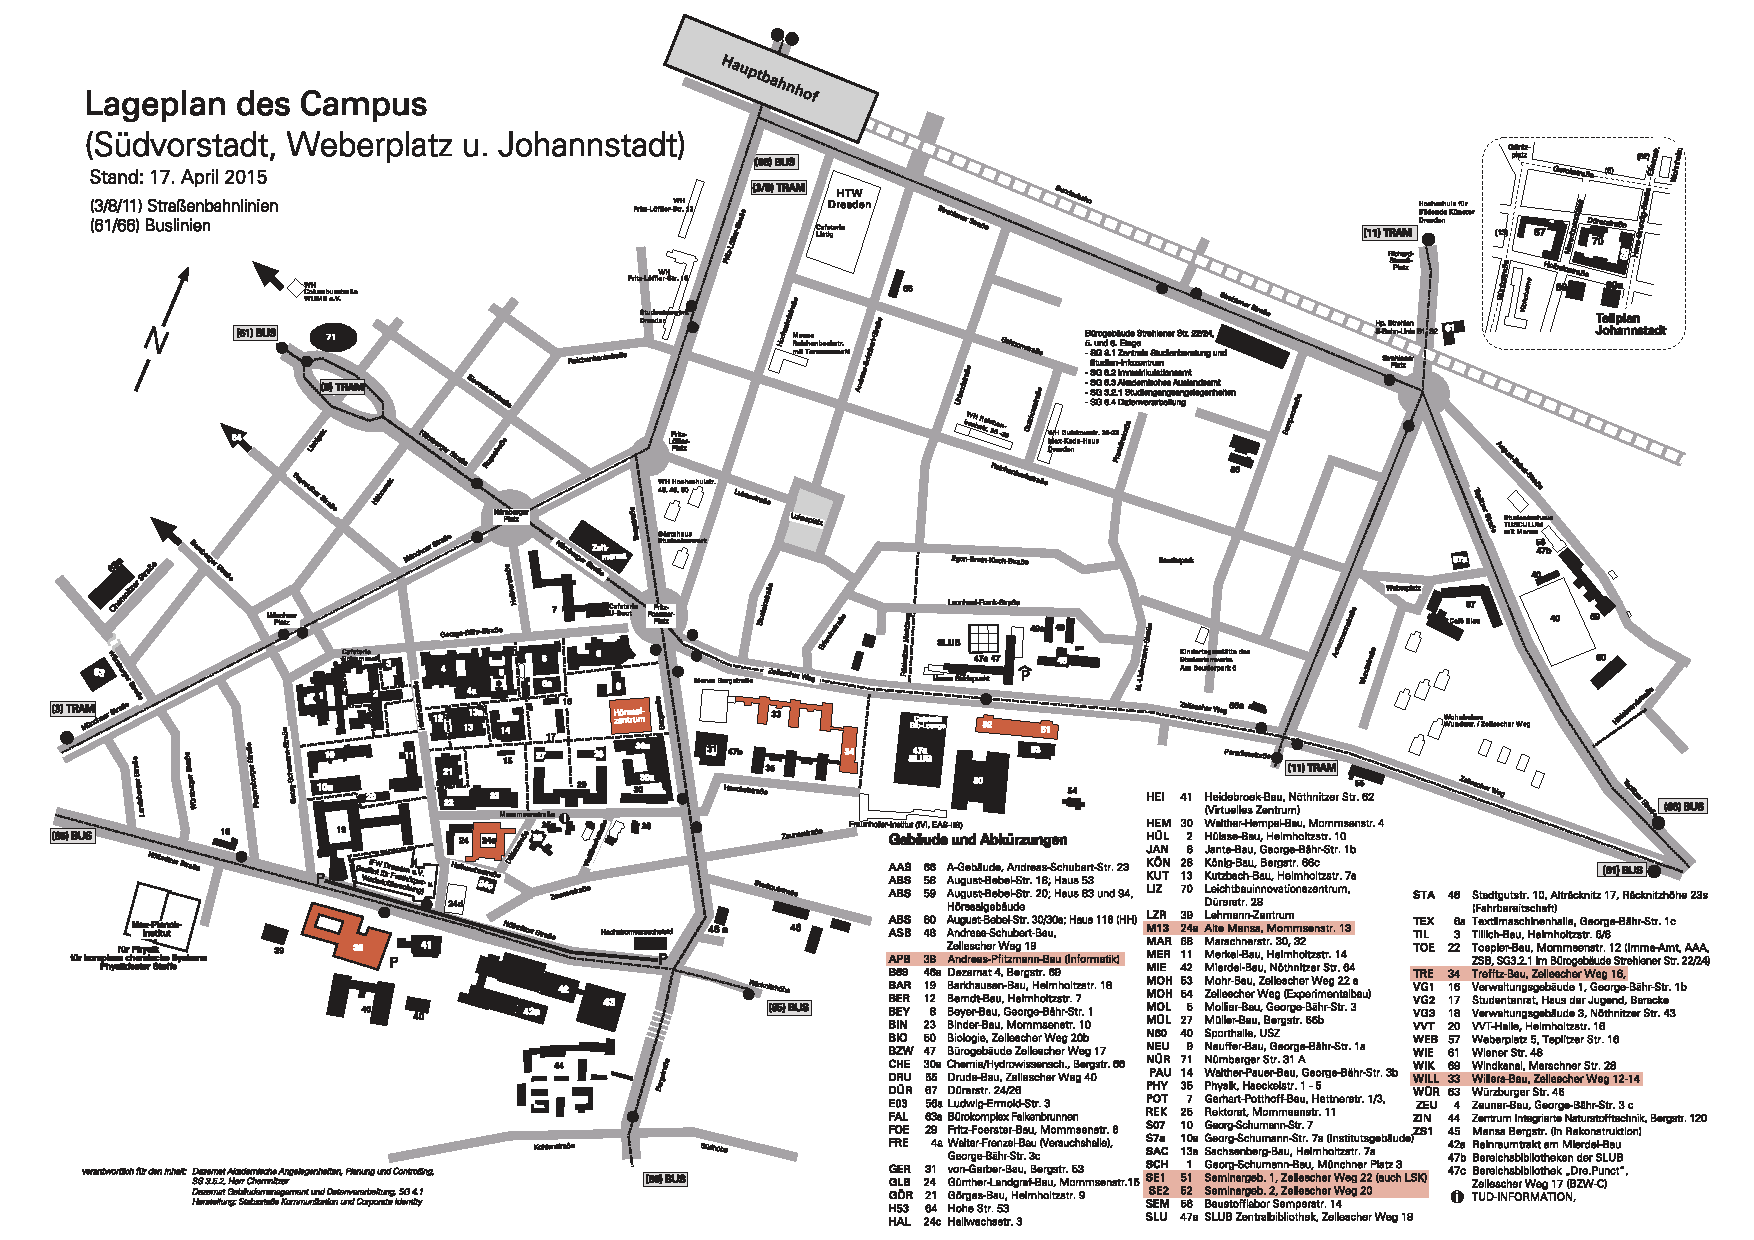
\includegraphics[width=\dimen107,height=\dimen108,keepaspectratio,trim=1.003\dimen107 0 0 0,clip]{img/campusplan_highlighted.pdf}%
\vfill
}}}
\mbox{}

\thispagestyle{empty}
\mbox{}
\newpage

\newpage
\thispagestyle{empty} %keine Seitenzahl
\color{white}

\begin{minipage}[t][\textheight][b]{.65\textwidth}
\footnotesize
\textbf{Herausgeber} \\
Fachschaftsrat Informatik der TU Dresden\\
Nöthnitzer Straße 46\\
01187 Dresden\\[1\baselineskip]

Alle verwendeten Comics von Randall Munroe (\textit{xkcd.com}) unter Creative Commons Lizenz:\\
\url{https://creativecommons.org/licenses/by-nc/2.5/}\\[1\baselineskip]

Redaktionsschluss dieser Ausgabe ist ein milder Spätsommerabend Mitte September 2019, noch vor dem Brexit.\\%[1\baselineskip]
Schwankungen im inhaltlichen Umfang sind technisch bedingt.\\[1\baselineskip]

Mitarbeit an der nächsten Version,\\
Verbesserungsvorschläge oder Tippfehlerfunde\\
sind unter \url{https://github.com/fsr/nopanic}\\
immer willkommen!\\[1\baselineskip]

Powered by \LaTeX
\end{minipage}%
\hfill%
\begin{minipage}[t][\textheight][b]{.25\textwidth}
\footnotesize
\raggedleft
\textbf{Dank an:}\\[1\baselineskip]
Amelie Wagner\\
Anees Hlaleh\\
Anita Fritzsche\\
Anja Reusch\\
Björn Glawe\\
Christina Ulonska\\
Eddy Loose\\
Fabian Wolf\\
Felix Wittwer\\
Florian Thie\\
Franka Schlösser\\
Jakob Behner\\
Jakob Krebs\\
Jannusch Bigge\\
Jeroen Trzaska\\
Katja Linnemann\\
Klaus-Rudolf Kladny\\
Lars Westermann\\
Laura Nagler\\
Lea Häusler\\
Leon Georgi\\
Lucas Hecht\\
Lucas Vogel\\
Lucian McIntyre\\
Marcel Legler\\
Michael Sippel\\
Nico Müller\\
Niklas Keerl\\
Nina Butz\\
Noemi Ernst\\
Oliver Scholz\\
Pascal Scholz\\
Patrik Phan\\
Philipp Niedergesäß\\
Rebecca Uecker\\
Robert Glöckner\\
Robert Ludwig\\
Robert Peine\\
Robert Ufer\\
Simon Birkenheuer\\
Tendsin Mende\\
Thorsten Seyschab\\
Tim Haering\\
Tobias Hänel\\
Tobias Maschek\\
Ulrich Huber\\
Verona Kolpe\\
Viktor Reusch
\end{minipage}

\enlargethispage{2\baselineskip}

\newcommand\BackcoverPic{%
\put(0,0){%
\parbox[b][\paperheight]{\paperwidth}{%
\vfill
\centering

\includegraphics[width = \paperwidth, height = \paperheight]{cover/Hinten}%
\vfill
}}}
\AddToShipoutPicture*{\BackcoverPic}


\end{document}
